\documentclass[letterpaper, 10 pt, conference]{ieeeconf}  % Comment this line out if you need a4paper
%\documentclass[a4paper, 10pt, conference]{ieeeconf}      % Use this line for a4 paper
\IEEEoverridecommandlockouts                              % This command is only needed if
\overrideIEEEmargins                                      % Needed to meet printer requirements.

%%%%%%%%%%%%%%%%%%%%%%%%%%%%%%%%%%%%%%%%%%%%%%%%%%%%%%%%%%%%%%%%%%%%%%%%%%%%%%%%

\usepackage{amsmath}
\usepackage{amssymb}
\usepackage{graphicx}
\usepackage{rotating}
\usepackage{xcolor}
\usepackage{tikz}
\usepackage{pgfplots}

%%%%%%%%%%%%%%%%%%%%%%%%%%%%%%%%%%%%%%%%

\DeclareMathOperator*{\argmin}{arg\,min}
\DeclareMathOperator*{\argmax}{arg\,max}
\DeclareMathOperator*{\vectorize}{vec}

\newcommand{\normal}[2]{\ensuremath{\mathcal{N}\left({{#1}},{{#2}}\right)}}
\newcommand{\trans}[1]{\ensuremath{{#1}^{\mathsf{T}}}}

\newcommand{\e}{\mathbf{e}}
\newcommand{\bb}{\mathbf{k}}
\newcommand{\kL}{\mathbf{k}^L}
\newcommand{\kG}{\mathbf{k}^G}
%\newcommand{\uu^m}{\mathbf{w}}
\newcommand{\x}{\mathbf{x}}
\newcommand{\y}{\mathbf{y}}
\newcommand{\uu}{\mathbf{u}}
\newcommand{\vv}{\mathbf{v}}
\newcommand{\timestep}{s}

\newcommand{\fixme}[1]{\textbf{FIXME: {#1}}}
\newcommand{\new}[1]{\color{red} {#1}}

\definecolor{darkgreen}{RGB}{0,127,0}

%%%%%%%%%%%%%%%%%%%%%%%%%%%%%%%%%%%%%%%%%%%%%%%%%%%%%%%%%%%%%%%%%%%%%%%%%%%%%%%%

\begin{filecontents}{paper.bib}
@inproceedings{wan2000unscented,
  title={The unscented Kalman filter for nonlinear estimation},
  author={Wan, Eric A and Van Der Merwe, Rudolph},
  booktitle={Adaptive Systems for Signal Processing, Communications, and Control Symposium 2000. AS-SPCC. The IEEE 2000},
  pages={153--158},
  year={2000},
  organization={Ieee}
}

@inproceedings{morelande2006reduced,
  title={Reduced sigma point filtering for partially linear models},
  author={Morelande, Mark R and Ristic, Branko},
  booktitle={2006 IEEE International Conference on Acoustics Speech and Signal Processing Proceedings},
  volume={3},
  pages={III--III},
  year={2006},
  organization={IEEE}
}

@inproceedings{padilla2010adaptive,
  title={An adaptive-covariance-rank algorithm for the unscented Kalman filter},
  author={Padilla, Lauren E and Rowley, Clarence W},
  booktitle={49th IEEE Conference on Decision and Control (CDC)},
  pages={1324--1329},
  year={2010},
  organization={IEEE}
}

@article{wang2010generating,
  title={Generating statistically correct random topologies for testing smart grid communication and control networks},
  author={Wang, Zhifang and Scaglione, Anna and Thomas, Robert J},
  journal={IEEE transactions on Smart Grid},
  volume={1},
  number={1},
  pages={28--39},
  year={2010},
  publisher={IEEE}
}

@inproceedings{hines2010topological,
  title={The topological and electrical structure of power grids},
  author={Hines, Paul and Blumsack, Seth and Sanchez, E Cotilla and Barrows, Clayton},
  booktitle={System Sciences (HICSS), 2010 43rd Hawaii International Conference on},
  pages={1--10},
  year={2010},
  organization={IEEE}
}


@article{schultz2014random,
  title={A random growth model for power grids and other spatially embedded infrastructure networks},
  author={Schultz, Paul and Heitzig, Jobst and Kurths, J{\"u}rgen},
  journal={The European Physical Journal Special Topics},
  volume={223},
  number={12},
  pages={2593--2610},
  year={2014},
  publisher={Springer}
}

@article{ghahremani2011online,
  title={Online state estimation of a synchronous generator using unscented Kalman filter from phasor measurements units},
  author={Ghahremani, Esmaeil and Kamwa, Innocent},
  journal={IEEE Transactions on Energy Conversion},
  volume={26},
  number={4},
  pages={1099--1108},
  year={2011},
  publisher={IEEE}
}

@article{ghahremani2016local,
  title={Local and wide-area pmu-based decentralized dynamic state estimation in multi-machine power systems},
  author={Ghahremani, Esmaeil and Kamwa, Innocent},
  journal={IEEE Transactions on Power Systems},
  volume={31},
  number={1},
  pages={547--562},
  year={2016},
  publisher={IEEE}
}

@article{ghahremani2011dynamic,
  title={Dynamic state estimation in power system by applying the extended Kalman filter with unknown inputs to phasor measurements},
  author={Ghahremani, Esmaeil and Kamwa, Innocent},
  journal={IEEE Transactions on Power Systems},
  volume={26},
  number={4},
  pages={2556--2566},
  year={2011},
  publisher={IEEE}
}

@article{wang2012alternative,
  title={An alternative method for power system dynamic state estimation based on unscented transform},
  author={Wang, Shaobu and Gao, Wenzhong and Meliopoulos, AP Sakis},
  journal={IEEE Transactions on Power Systems},
  volume={27},
  number={2},
  pages={942--950},
  year={2012},
  publisher={IEEE}
}

@article{qing2015decentralized,
  title={Decentralized unscented Kalman filter based on a consensus algorithm for multi-area dynamic state estimation in power systems},
  author={Qing, Xiangyun and Karimi, Hamid Reza and Niu, Yugang and Wang, Xingyu},
  journal={International Journal of Electrical Power \& Energy Systems},
  volume={65},
  pages={26--33},
  year={2015},
  publisher={Elsevier}
}

@article{rigatos2013distributed,
  title={A distributed state estimation approach to condition monitoring of nonlinear electric power systems},
  author={Rigatos, G and Siano, Q and Zervos, N},
  journal={Asian Journal of Control},
  volume={15},
  number={3},
  pages={849--860},
  year={2013},
  publisher={Wiley Online Library}
}

@article{yang2013false,
  title={On false data injection attacks against Kalman filtering in power system dynamic state estimation},
  author={Yang, Qingyu and Chang, Liguo and Yu, Wei},
  journal={Security and Communication Networks},
  year={2013},
  publisher={Wiley Online Library}
}

@incollection{witczak2014unknown,
  title={Unknown Input Observers and Filters},
  author={Witczak, Marcin},
  booktitle={Fault Diagnosis and Fault-Tolerant Control Strategies for Non-Linear Systems},
  pages={19--56},
  year={2014},
  publisher={Springer}
}

@article{bolandhemmat2012solution,
  title={A Solution to the State Estimation Problem of Systems with Unknown Inputs},
  author={Bolandhemmat, Hamidreza and Clark, Christopher and Golnaraghi, Farid},
  journal={Recent Patents on Mechanical Engineering},
  volume={5},
  number={2},
  pages={102--112},
  year={2012},
  publisher={Bentham Science Publishers}
}

@article{yang1988observers,
  title={Observers for linear systems with unknown inputs},
  author={Yang, Fuyu and Wilde, Richard W},
  journal={IEEE transactions on automatic control},
  volume={33},
  number={7},
  pages={677--681},
  year={1988},
  publisher={Institute of Electrical and Electronics Engineers}
}

@inproceedings{amini2015dynamic,
  title={Dynamic load altering attacks in smart grid},
  author={Amini, Sajjad and Mohsenian-Rad, Hamed and Pasqualetti, Fabio},
  booktitle={Innovative Smart Grid Technologies Conference (ISGT), 2015 IEEE Power \& Energy Society},
  pages={1--5},
  year={2015},
  organization={IEEE}
}

@inproceedings{amini2015detecting,
  title={Detecting dynamic load altering attacks: A data-driven time-frequency analysis},
  author={Amini, Sajjad and Pasqualetti, Fabio and Mohsenian-Rad, Hamed},
  booktitle={2015 IEEE International Conference on Smart Grid Communications (SmartGridComm)},
  pages={503--508},
  year={2015},
  organization={IEEE}
}

@article{fang2012smart,
  title={Smart grid�The new and improved power grid: A survey},
  author={Fang, Xi and Misra, Satyajayant and Xue, Guoliang and Yang, Dejun},
  journal={IEEE communications surveys \& tutorials},
  volume={14},
  number={4},
  pages={944--980},
  year={2012},
  publisher={IEEE}
}

@article{wang2009cascade,
  title={Cascade-based attack vulnerability on the US power grid},
  author={Wang, Jian-Wei and Rong, Li-Li},
  journal={Safety Science},
  volume={47},
  number={10},
  pages={1332--1336},
  year={2009},
  publisher={Elsevier}
}

@article{rosas2007topological,
  title={Topological vulnerability of the European power grid under errors and attacks},
  author={Rosas-Casals, Marti and Valverde, Sergi and Sol{\'e}, Ricard V},
  journal={International Journal of Bifurcation and Chaos},
  volume={17},
  number={07},
  pages={2465--2475},
  year={2007},
  publisher={World Scientific}
}

@article{albert2004structural,
  title={Structural vulnerability of the North American power grid},
  author={Albert, R{\'e}ka and Albert, Istv{\'a}n and Nakarado, Gary L},
  journal={Physical review E},
  volume={69},
  number={2},
  pages={025103},
  year={2004},
  publisher={APS}
}

@Article{FRL1,
author = {A.~Molina-Garcia� and F.~Bouffard and D.~S.~Kirschen},
title = {Decentralized Demand-Side Contribution to Primary Frequency Control},
journal = {IEEE Trans. on Power Systems},
volume = 26,
number = 1,
pages = {411-419},
month = feb,
year = 2011
}

@Article{FRL2,
author = {J.~A.~Short and D.~G.~Infield and L.~L.~Freris},
title = {Stabilization of Grid Frequency Through Dynamic Demand Control},
journal = {IEEE Trans. on Power Systems},
volume = 22,
number = 3,
pages = {1284-1293},
month = aug,
year = 2007
}

@Article{FRL3,
author = {C.~Zhao and U.~Topcu and S.~H.~Low},
title = {Optimal Load Control via Frequency Measurement and Neighborhood Area Communication},
journal = {IEEE Trans. on Power Systems},
volume = 28,
number = 4,
pages = {3576-3587},
month = nov,
year = 2013
}

@inproceedings{Pasqualetti2012,
  title={Cyber-physical security via geometric control: Distributed monitoring and malicious attacks},
  author={Pasqualetti, Fabio and D{\"o}rfler, Florian and Bullo, Francesco},
  booktitle={2012 IEEE 51st IEEE Conference on Decision and Control (CDC)},
  pages={3418--3425},
  year={2012},
  organization={IEEE}
}

@inproceedings{Demarco1996,
  title={The potential for malicious control in a competitive power systems environment},
  author={DeMarco, Christopher L and Sariashkar, JV and Alvarado, Fernando},
  booktitle={Control Applications, 1996., Proceedings of the 1996 IEEE International Conference on},
  pages={462--467},
  year={1996},
  organization={IEEE}
}

@article{Mohsenian-Rad2010,
  title={Distributed internet-based load altering attacks against smart power grids},
  author={Mohsenian-Rad, Amir-Hamed and Leon-Garcia, Alberto},
  journal={IEEE Transactions on Smart Grid},
  volume={2},
  number={4},
  pages={667--674},
  year={2011},
  publisher={IEEE}
}

@article{Marnerides2014,
  title={Power consumption profiling using energy time-frequency distributions in smart grids},
  author={Marnerides, Angelos K and Smith, Paul and Schaeffer-Filho, Alberto and Mauthe, Andreas},
  journal={IEEE Communications Letters},
  volume={19},
  number={1},
  pages={46--49},
  year={2015},
  publisher={IEEE}
}
\end{filecontents}
\immediate\write18{bibtex paper}

%%%%%%%%%%%%%%%%%%%%%%%%%%%%%%%%%%%%%%%%%%%%%%%%%%%%%%%%%%%%%%%%%%%%%%%%%%%%%%%%


\title{\LARGE \bf
    Identification of Destabilizing Attacks in Power Systems
    \thanks{The authors are with the Bourns College of Engineering, University of California, Riverside, CA, USA.
    This work was supported in part by the National Science Foundation (NSF) grant ECCS/AFOSR  1462530.}
}

\author{ Mike Izbicki, Sajjad Amini, Christian Shelton, and Hamed Mohsenian-Rad}
%\author{Albert Author$^{1}$ and Bernard D. Researcher$^{2}$% <-this % stops a space
%\thanks{*This work was not supported by any organization}% <-this % stops a space
%\thanks{$^{1}$Albert Author is with Faculty of Electrical Engineering, Mathematics and Computer Science,
        %University of Twente, 7500 AE Enschede, The Netherlands
        %{\tt\small albert.author@papercept.net}}%
%\thanks{$^{2}$Bernard D. Researcheris with the Department of Electrical Engineering, Wright State University,
        %Dayton, OH 45435, USA
        %{\tt\small b.d.researcher@ieee.org}}%
%}


\begin{document}



\maketitle
\thispagestyle{empty}
\pagestyle{empty}

%%%%%%%%%%%%%%%%%%%%%%%%%%%%%%%%%%%%%%%%%%%%%%%%%%%%%%%%%%%%%%%%%%%%%%%%%%%%%%%%
\begin{abstract}
In a destabilizing attack against power systems, the adversary hacks into the generator or load control mechanisms to insert positive feedback into power system dynamics. The implementation of destabilizing attacks, both on the generation and load sides, have recently been studied. There are also recent advances on how to detect, i.e., realize the presence of, destabilizing attacks in power systems. However, identifying the location(s) of the compromised buses is still an open problem. This is particularly challenging if, as in practice, one does not even know the number of compromised buses. Another challenge is to keep low computational complexity to allow fast attack identification with high accuracy. To address these various issues,
%
% form insert positive feedback into a power system.
%This feedback destabilizes the system by changing the power system dynamics,
%which can damage equipment.
%In this paper, we propose a method for detecting destabilizing attacks.
we observe in this paper that destabilizing attacks can be modeled as a reparameterization of the power system's dynamical model. Therefore, we propose an attack detection method that uses the Unscented Kalman Filter to jointly estimate both the system states and parameters of the attack.
We also propose a low-rank modification to the Kalman filter that improves computational efficiency while maintaining accuracy of detection.
We show empirically that this method successfully identifies complex attacks involving many buses.
\end{abstract}


%%%%%%%%%%%%%%%%%%%%%%%%%%%%%%%%%%%%%%%%%%%%%%%%%%%%%%%%%%%%%%%%%%%%%%%%%%%%%%%%
\section{Introduction}

In this paper, we consider attacks against power system stability. Such attacks can be conducted in different ways, either on the generation side \cite{Pasqualetti2012, Demarco1996} or on the load side \cite{Mohsenian-Rad2010, Marnerides2014, amini2015dynamic}. Either way it essentially involves inserting positive feedback into the various power system control mechanisms.

Recent work has made advances on how to \emph{detect}, i.e., realize the presence of, destabilizing attacks in power systems. Specifically, in \cite{amini2015detecting}, a detection methodology is proposed that works based on applying fast fourier transform (FFT) to system measurements. It uses the fact that a destabilizing attack will introduce new frequencies into the FFT that are not present during normal operation. Therefore, the presence of such new frequencies beyond certain pre-specified magnitude thresholds indicate the presence of a destabilizing attack.

In this paper, we move one step ahead and address the open problem of \emph{identifying} destabilizing attacks against power systems by only monitoring state variables. That is, we devise a method that examines the state variables data from power system sensors such as phasor measurement units (PMUs) to indicate at which exact power system buses (i.e., nodes) the load and/or generation are compromised.

Our proposed method has three main properties:

\begin{enumerate}

\item It does not require prior knowledge on the number of buses that are compromised. That is, as in practice, we assume that the grid operator is not initially aware of how many buses are compromised. Nevertheless, our method can identify which buses are compromised.

\item Prior methods, e.g., in \cite{amini2015detecting}, often analyze the attack at each individual bus, which would allow attack identification only if the method is applied several times separately on every bus. In contrast, our method naturally identifies attacks on the entire system considered as a whole. This reduces the computation time.

\item It is capable of distinguishing destabilizing attacks, i.e., load or generation control loops that are malicious and based on positive feedback, from the many load and generation control loops that exist in a power system that are benign and based on negative feedback.

\end{enumerate}

The main tool that we use in this paper is the Unscented Kalman Filter (UKF) to perform dual state estimation to estimate an unknown attack matrix. We then identify the attack location(s) through a proper thresholding mechanism applied to the entries of the estimated attack matrix.



%The contributions in this paper can be summarized as follows:
%



%On the generation side, the attack might compromise the generator governor controller directly or the generator's sensors and communications systems. See \cite{Pasqualetti2012, Demarco1996} for more details and examples. On the load side, the attack might compromise the direct or indirect load control mechanisms, e.g., in demand response programs, or their associated sensors, or command signals. See \cite{Mohsenian-Rad2010, Marnerides2014, amini2015dynamic} for more details.


%One of the most common methods for inserting positive feedback is manipulating load consumption by getting feedback from frequency through a simple proportional gain controller.
%\fixme{We need to at least list some other attack types.} This is known as a dynamic load altering attack \cite{}. We aim to detect the presence of such attacks and identify  their type, e.g. compromised loads in dynamic load altering attacks.

%Recent work has made advances on how to detect these attacks \cite{amini2015dynamic,amini2015detecting}. This prior work has several limitations that are fixed in this paper:
%\begin{enumerate}
%\item
%Prior work is concerned only with identifying attacks on an individual bus.
%To identify attacks on the entire system, the method must be run several times separately on every bus.
%%This complicates the procedure's implementation and increases computational complexity.
%Our method naturally identifies attacks on the entire system considered as a whole.
%This reduces the identification time.
%\fixme{We need a definition of detection vs identification.}
%\item
%Prior work can only determine that feedback has been added to the system;
%it provides no information about the \emph{sign} nor \emph{magnitude} of the attack.
%Our method estimates both.
%This information is useful when deciding which countermeasures to take to mitigate the effectiveness of the attack.
%%Estimating the magnitude can be important for determining the severity of the attack and deciding the appropriate corrective measures.
%\end{enumerate}

\subsection{Related work}
%\fixme{This section is basically just a list of possibly related papers.}

%There exist good filtering methods for designing Unknown Input Observers (UIOs).
%\cite{yang1988observers,bolandhemmat2012solution,witczak2014unknown}
%Using one of these methods, we can estimate the control input for our system,
%then apply the previous techniques to detect attacks.
%The UIO technique introduces extra overhead steps, however.
%My technique estimates the attack directly without needing to first estimate the control input.




This paper belongs to the family of studies that address destabilizing attacks against power systems. While the focus so far has been mostly on the definition and implementation of such attacks \cite{Demarco1996, Mohsenian-Rad2010, amini2015dynamic}, on the methods to protect the power system against such attacks \cite{Pasqualetti2012, AminiJournal2015, Marnerides2014}, and occasionally on methods to detect such attacks \cite{amini2015detecting}, the focus in this paper is on the less explored topic of identifying the attack by finding the location(s) of the compromised buses.

In terms of the methodology that is used in this paper, the UKF has been used before for power system problems, e.g., in \cite{ghahremani2011online} to estimate the rotor angle and speed in synchronous generators. However, no joint estimation is used, and the system is not under attack. A more recent analysis is presented in \cite{ghahremani2016local} to estimate the parameters of the motor controller and bus loads. Again, the system is not under attack.

%\cite{ghahremani2011dynamic}
%Another EKF-UI paper by the same authors.
%\cite{ghahremani2016local}

This paper shows through numerical results that the current power system monitoring systems would require calculation of a large Jacobian matrix if one wants to apply the UKF without modification for the purpose of identifying destabilizing attacks. In this regard, the current study is related also to a thread of work, such as in \cite{wang2012alternative, qing2015decentralized}, that similarly have to deal with the computational issues that arise when applying the UKF to power systems. Again, these studies do not address the power system under attack and the details of the analysis are different from those in this paper.


%They propose using the UKF to avoid the need for a Jacobian, both improving runtime and accuracy.
%\cite{wang2012alternative}
%This paper claims that using the UKF to monitor realworld power systems is too slow.
%They identify two bottlenecks to a centralized monitor.
%First, there is a lot of communication required from every node to the monitor.
%Second, the monitor must do a lot of computation.
%They solve both problems by partitioning the powergrid into disjoint smaller grids,
%filtering each grid independently,
%and carefully communicating the results between the smaller grids.
%A similar technique might be useful to speed up my solution,
%but this is a different idea than I had.
%\cite{qing2015decentralized}
%This paper also does a distributed analysis of realworld power systems as above.
%This paper is more similar to our paper because they are specifically looking to detect faults.
%They detect faults in a different way.
%We have a specific model of the way faults are generated that we are looking to detect by adding new states to the system.
%They do not have a specific model, and instead apply a function to the existing states in an attempt to detect faults.
%\cite{rigatos2013distributed}


\section{Problem statement}


\begin{figure}
\centering
\begin{tikzpicture}
\small

%\node at (0,10) {};
\node at (0,4.75) {
    \begin{tikzpicture}
    \begin{axis}
        [ domain=-30:80
        , xmin=-30
        , xmax=80
        , ymin=-2000
        , ymax=2000
        , width=0.55\textwidth
        , height=1.5in
        , samples=500
        , xtickmin=1,xtickmax=0,ytickmin=1,ytickmax=0, minor tick num=0, scaled ticks=false, xticklabel=\empty,yticklabel=\empty
        ]
    \draw[ultra thin,opacity=0.2] (axis cs:\pgfkeysvalueof{/pgfplots/xmin},0) -- (axis cs:\pgfkeysvalueof{/pgfplots/xmax},0);
    \draw[ultra thin,opacity=1.2,red] (axis cs:0,\pgfkeysvalueof{/pgfplots/ymin}) -- (axis cs:0,\pgfkeysvalueof{/pgfplots/ymax});
    \addplot[color=blue,mark=none] {(\x>0)*x^(1.75)*sin(deg(x))};
    \end{axis}

    \node at (4.55,1.55) {\color{blue} $\omega_2$};
    \node at (1.1,1.6) {\color{red} attack begins};
    \draw[red,->] (2,1.6) -- (2.2,1.6);

    \draw[fill=green,draw opacity=0,fill opacity=0.05] (0,0.3) -- (8.20,0.3) -- (8.20,1.95) -- (0,1.95);
    \draw[dashed,darkgreen] (0,0.3) -- (8.2,0.3);
    \draw[dashed,darkgreen] (8.2,1.95) -- (0,1.95);

    \node at (4.25,0.5) {\color{darkgreen} safe operating range};

    %\node at (
    \end{tikzpicture}
};

\node at (0,0) {
    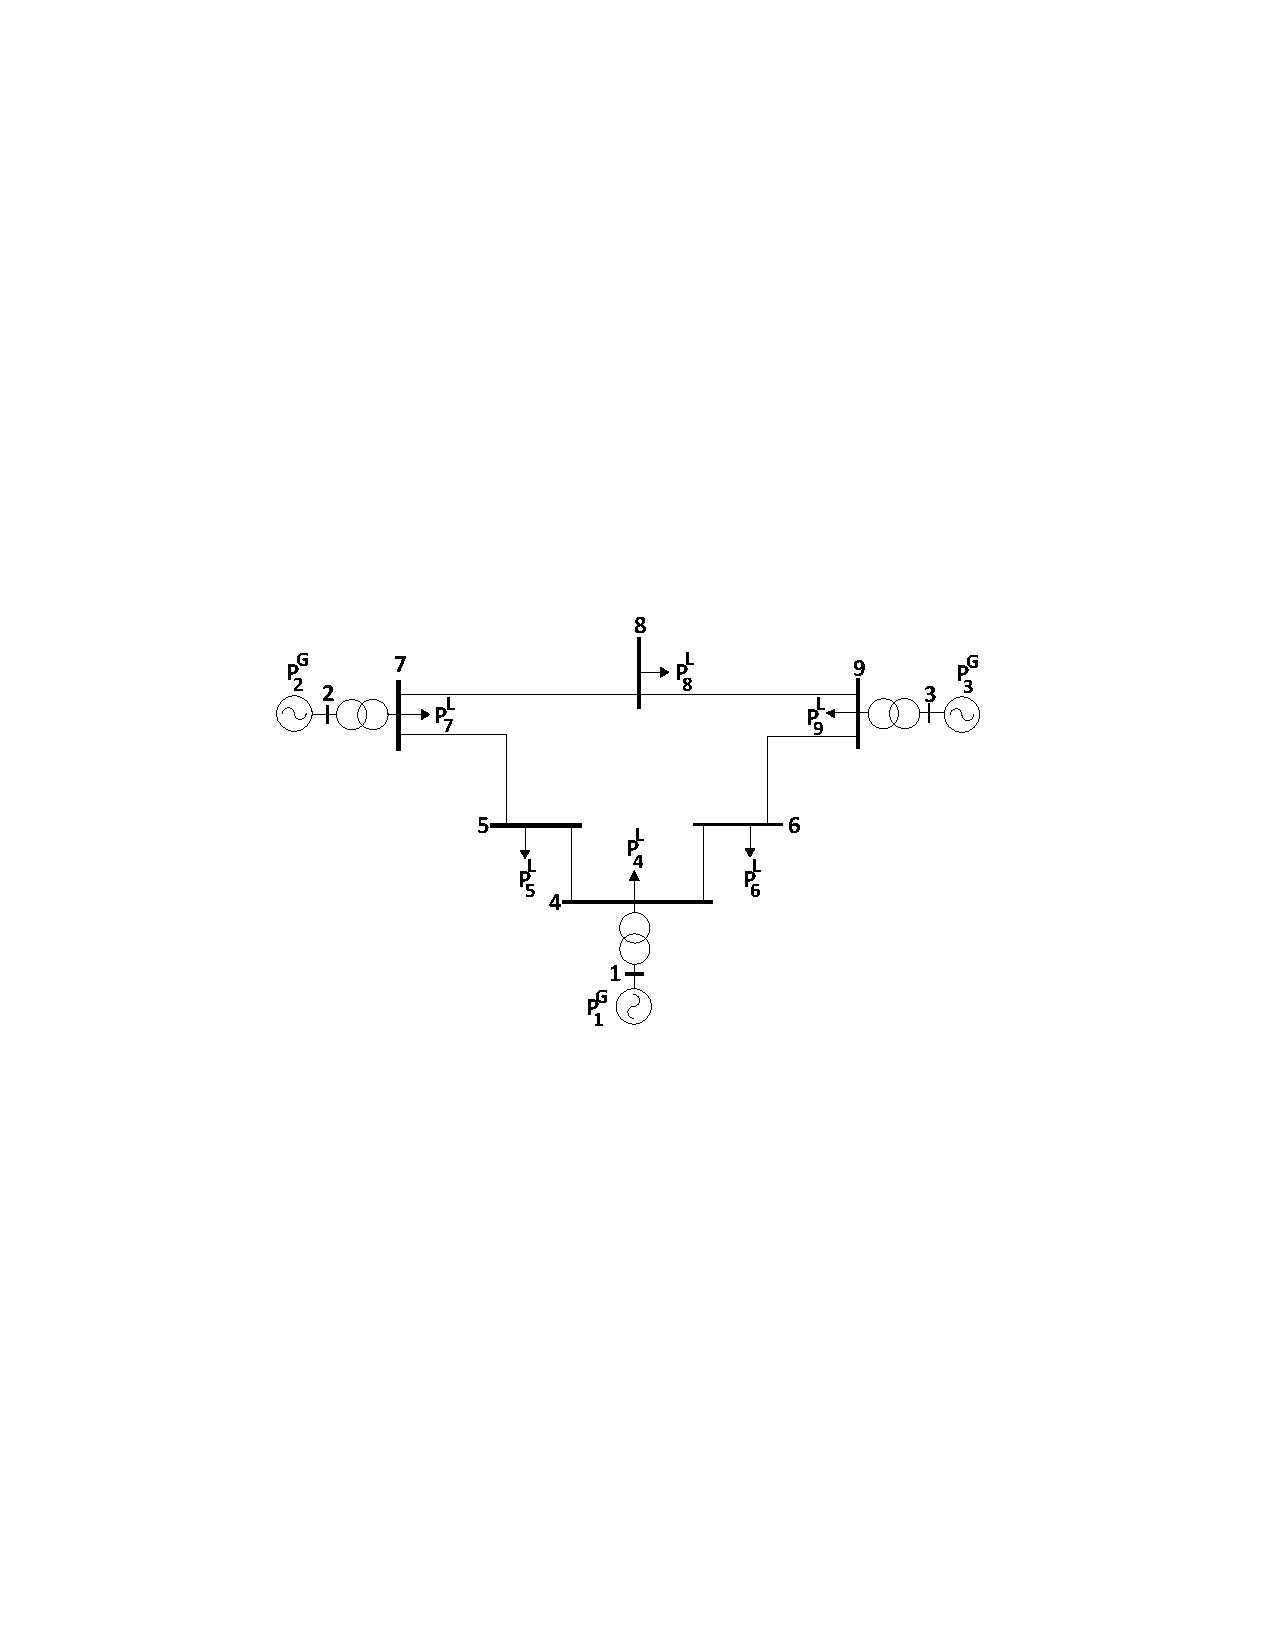
\includegraphics[width=0.43\textwidth]{img/IEEE9}
};

\draw[blue,line width=0.25pt,fill,draw opacity=0.5,fill opacity=0.1]
    (-3.95,0.8) -- (-2.75,0.8) -- (-2.75,1.9) -- (-3.95,1.9) -- cycle;

\draw[dotted,thick] (-3.95,1.9) -- (-4.1,3.6);
\draw[dotted,thick] (-2.75,1.9) -- (4.1,3.6);

\node[draw=red,fill=red,fill opacity=0.05,circle,minimum width=1.5cm] (8) at (0.25,1.6) {};
\node[draw=red,fill=red,fill opacity=0.05,circle,minimum width=1.5cm] (3) at (3.5,1.25) {};
\draw[red,thick,->] (8) to[out=20,in=120] (3);

\end{tikzpicture}
\caption{
    The standard IEEE 9 bus power system under a destabilizing attack.
    The attacker has added a load to bus 8 that gets positive feedback from generator bus 3.
    This causes instabilities throughout the power system.
    The inset shows that generator 2's rotar angle frequency deviation ($\omega_2$).
    During normal operations, $\omega_2$ remains close to 0 because the system is stable.
    The attack adds instability to the system, which causes $\omega_2$ to exceed safe operating levels unless corrective action is taken.
    Our goal is to identify which system buses are compromised so that we can take this corrective action.
}

\label{fig:example}
\end{figure}

We consider a power system with $g$ generator buses and $\ell$ load buses.
An example is shown in Figure \ref{fig:example}.
We model the dynamics of this system using the standard linear power system state space equation
\begin{equation}
\dot\x = A\x + B\uu
,
\label{sys:norm}
\end{equation}
where the state variables and inputs are
\begin{align}
\x
=
\begin{bmatrix} \delta \\ \theta \\ \omega \end{bmatrix}
,
~~~\uu
=
\begin{bmatrix} P^G \\ P^L \end{bmatrix}
.
\end{align}
Here,
$\delta$ is the vector of voltage phase angles at all generator buses,
$\omega$ is the vector of rotor angular frequency deviations at all generator buses,
$\theta$ is the vector of voltage phase angles at all load buses,
$P^L$ is the vector of power consumption at all load buses,
and $P^G$ is the vector of power generation at all generator buses.
Many generators are equipped with Automatic Generation Control (AGC),
which is a system for automatically adjusting the power output in response to the load.
Entries of $P^G$ associated with generators that have AGC are zero.
All other entries are nonzero.
The system dynamics matrices are
%\resizebox{0.4\textwidth}{!}{
\newcommand{\negone}{\scalebox{0.95}{-}1}
\begin{align*}
\hspace{-0.3in}
A
\!\!&=\!\!\!
\begin{bmatrix}
0 & 0 & I
\\
%(D^L)^{-1}H^{LG} & (D^L)^{-1}H^{LL} & -(D^L)^{-1}K^{LG}
(D^L)^{\negone}H^{LG} & (D^L)^{\negone}H^{LL} & 0
\\
-M^{\negone}(K^I\!\!+\!\! H^{GG}) & -M^{\negone}H^{GL} & -M^{\negone}(K^P\!\!\!+\!\!D^G)
\end{bmatrix}
,
%\end{align*}
%\begin{flalign*}
\\
B
%&=
\!\!&=\!\!\!
\begin{bmatrix}
0 & 0
\\
0 & (D^L)^{\negone}
\\
-M^{\negone} & 0
\end{bmatrix}
,
%&
\end{align*}
%}
where
$I$ is the identity matrix of appropriate dimension,
and $M$, $D^G$, and $D^L$ are diagonal matrices with diagonal entries equal to the inertia, damping coefficients of generators, and damping coefficients of loads, respectively.
Matrices $H^{LG}$, $H^{GG}$, $H^{GL}$, and $H^{LL}$ are the imaginary components of the standard system admittance matrix $H^{bus}$.
Specifically,
\begin{align*}
  H^{bus} =
  \begin{bmatrix}
    H^{GG} & H^{GL} \\
    H^{LG} & H^{LL}
  \end{bmatrix}.
\end{align*}
Matrices $K^I$ and $K^P$ are diagonal matrices with diagonal entries equal to the integral and proportional coefficients of the generator controllers with AGC capability.
Note that the coefficients corresponding to generators without AGC are zero.
This system incorporates the swing equations for generators, power flow equations for the transmission network, and the governor and load frequency controller for generators with AGC.

The focus in this paper is attacks against power system stability.
As shown in Figure \ref{fig:example},
an attack in one portion of the power system can cause instability throughout the power system.
These destabilizing attacks can affect both generation and load sectors.
On the generation side, the attack might compromise the generator governor controller directly or the generator's sensors and communications systems.
(See \cite{Pasqualetti2012, Demarco1996} for more details.)
On the load side, the attack might compromise the direct or indirect load control mechanisms, e.g., in demand response programs, or their associated sensors, or command signals.
(See \cite{Mohsenian-Rad2010, Marnerides2014, amini2015dynamic} for more details.)
In either case, the attacker's goal is to insert positive feedback into the system.

We model a destabilizing attack by decomposing the control input vector $\uu$ as
\begin{equation}
\label{eq:una}
\uu = \uu^n + \uu^a
.
%,~~~
%\uu^n
%=
%\begin{bmatrix} P^{Gn} \\ P^{Ln} \end{bmatrix}
%,~~~
%\uu^a
%=
%\begin{bmatrix} P^{Ga} \\ P^{La} \end{bmatrix}
\end{equation}
Here, the vector $\uu^n$ denotes the control input under normal operation
and the vector $\uu^a$ represents the control input added by the attacker.
%where the $n$ superscript denotes the control input under normal operation and the $a$ superscript represents the input added by the attacker.
%Here, the vector $\uu^a$ denotes the portion of the system input generated by the attacker.
%The portion of the attack implemented on the generation side is represented by the compromised power injection vector $P^{Ga}$.
%Similarly, the portion of the attack implemented on the load side is represented by the compromised power consumption vector $P^{Ga}$.
%The new power system dynamics under a simple destabilizing attack with proportional positive feedback gains can be expressed as:
%Substituting Equation \ref{eq:una} into Equation \ref{sys:norm} gives the dynamics of the power system under attack:
%\begin{equation}
%\label{sys:attack1}
%\dot\x = A\x + B(\uu^n + \uu^a)
%.
%\end{equation}
%where
%\begin{equation}
%\uu^a =
%\begin{bmatrix}P^{Ga}\\P^{La}\end{bmatrix}
%.
%\end{equation}
%the vectors $P^{Ga}$ and $P^{La}$ (and hence $\uu^a$) represent loads added to the system by the attacker.
%All three vectors are allowed to vary over time.
%When no attack is present, $\uu^a$ is zero, and the system above reduces to Equation \ref{sys:norm}.
%In a static load altering attack, the attack input $\uu^a$ remains a constant non-zero value throughout the attack.
%Static attacks can introduce transients into the system,
%but they cannot destabilize the system.
%In a dynamic load altering attack, $\uu^a$ changes over time.
%Relatively small changes in $\uu^a$ can induce large, destabilizing changes in the system.
%This makes dynamic load altering attacks much more dangerous than their static counterparts.
We consider the case where the attacker uses a proportional controller to dynamically determine the value of $\uu^a$ with feedback taken from the demand side.
Loads with this feedback are called \emph{frequency-responsive controllable loads}, and are widely used in practice \cite{FRL1, FRL2, FRL3}.
We model the proportional controller input vector as
\begin{equation}
\label{eq:pos}
\uu^a = A^p\x + \uu^p
,
\end{equation}
%The input $\uu^p$ is assumed to remain constant throughout the attack,
%but $A^p$ is allowed to vary over time.
%In this scheme, the compromised load vector can be decomposed as
%Since our proportional controller is frequency responsive, we can decompose the $A^p$ matrix as
where
\begin{equation}
A^p =
\begin{bmatrix}
%0 & 0 & 0
%\\
0 & 0 & -(D^L)^{-1}K^{LG}
\\
0 & 0 & 0
\end{bmatrix}
.
\end{equation}
The entry in row $i$ column $j$ of matrix $K^{LG}$ contains the proportional gain for load bus $i$ getting feedback from the frequency of generator bus $j$.
If the entry is positive, then bus $i$ is under attack and the system may destabilize.
If the entry is negative, then there is a benign frequency-responsive load.
These loads will never destabilize the system.
If the entry is zero, there are no frequency-responsive loads.
Substituting \eqref{eq:pos} and \eqref{eq:una} into \eqref{sys:norm} gives us our final system dynamics under attack:
\begin{equation}
\label{sys:attack2}
\begin{aligned}
\dot\x &= (A + BA^p)\x + B(\uu^n + \uu^p)
.
\end{aligned}
\end{equation}
The attack will be destabilizing if the maximum eigenvalue of $(A+BA^p)$ is greater than 1.

Detecting the presence of an attack is not difficult.
It can be done by monitoring only a few state variables \cite{amini2015dynamic}.
However, identifying which load bus is compromised is an open problem.
In this paper, we propose an identification method that directly estimates the $K^{LG}$ matrix.
Our method automatically determines which load buses are compromised and can distinguish between destabilizing and benign loads.
Our method requires access only to synchronized measurements of the state vector $\x$,
and does not require access to the control input $\uu$.
These state measurements are widely available in existing modern power systems through Phasor Measurement Units (PMUs).

%%%%%%%%%%%%%%%%%%%%%%%%%%%%%%%%%%%%%%%%

\section{Attack Identification Method} \label{sec:method}
\label{sec:method}

Our attack identification procedure has two steps.
First we estimate the $K^{LG}$ matrix using \emph{dual state estimation}.
This is a standard technique that applies the Unscented Kalman Filter (UKF) \cite{wan2000unscented} to simultaneously estimate the entries of matrix $K^{LG}$ and the system states $\x$.
Unfortunately, the standard application of this technique does not work well for our problem.
It is too slow computationally and has poor accuracy.
So we introduce a novel rank-1 approximation which lets us effectively apply dual state estimation to our problem.
Finally, once $K_{LG}$ is estimated, we apply a thresholding procedure to identify the attacked buses.

\subsection{Standard dual state estimation and its limitations}
%Dual state estimation is a standard technique for estimating a dynamical system's parameters at the same time as we estimate the state.
%It is traditionally described using the system's discrete state equations.
%We describe the naive application of dual state estimation and its limitations with respect to our problem.
Dual state estimation is traditionally described using the system's discrete state equations,
so we begin our presentation by discretizing \eqref{sys:attack2} as
\begin{equation}
\label{eq:discrete}
\x_{t+1} = (\timestep A+sBA^p_t+I)\x_t + \timestep B(\uu_t^n+\uu_t^p) + \epsilon.
\end{equation}
The subscripts indicate the timestep,
$\timestep$ is a scalar that represents the length of a time step,
and $\epsilon \sim \normal{0}{Q^\epsilon}$ is an error term capturing both modeling and observation errors.

Now we describe how to estimate the $A^p_t$ matrix.
Recall that in the definition of $A^p_t$,
the $K^{LG}_t$ matrix is unknown and determined by the attacker;
all other elements are statically known.
%Therefore, to estimate $A^p_t$, it is sufficient to estimate $K^{LG}_t$.
%We can estimate $K^{LG}_t$ directly using dual state estimation.
In dual state estimation, we augment the original dynamical system's state variables to also include the elements of $K^{LG}_t$.
The resulting augmented system is
\begin{equation}
\label{eq:aug}
\begin{aligned}
\begin{split}
\begin{bmatrix}
\x_{t+1} \\
\vectorize K^{LG}_{t+1}
\end{bmatrix}
&=
\begin{bmatrix}
sA + sBA^p_t + I & 0 \\
0 & I
\end{bmatrix}
\begin{bmatrix}
\x_t \\
\vectorize K^{LG}_t
\end{bmatrix}
\\&~~~~~~~~~~+
\begin{bmatrix}
sB & 0\\
0 & I
\end{bmatrix}
\begin{bmatrix}
\uu_t^n + \uu_t^p \\
\uu^m_t
\end{bmatrix}
+
\begin{bmatrix}
\epsilon \\
\epsilon^m
\end{bmatrix}
\end{split}
,
\end{aligned}
\end{equation}
where
\begin{equation}
\epsilon \sim \normal{0}{Q^\epsilon}
%~~~~~~~~~~~~~~~~~~~~~~~~~~~~~~~~~
%\\
,~~~
\epsilon^m\sim\normal{0}{Q^{\epsilon^m}}
%~~~~~~~~~~~~~~~~~~~~~~~~~~~~~~
\label{sys:dualized}
\end{equation}
Here we have also introduced a new control input $\uu^m_t$ with error $\epsilon_m$.
It is unobserved and controlled by the attacker.
Specifically, the attacker uses $\uu^m_t$ to manipulate the entries of $K^{LG}_t$, and hence $A^p_t$.
The notation $\vectorize K^{LG}_t$ refers to the column vector constructed by stacking the columns of $K^{LG}_t$ on top of each other.

Next we note that the control inputs $\uu^n_t$, $\uu^a_t$, and $\uu^m_t$ are unobserved.
A standard technique for modeling unobserved inputs is to replace them with random error terms.
%In particular, we assume $\uu^n_t\sim\normal{0}{Q^n}$, $\uu^a_t\sim\normal{0}{Q^a}$, and $\uu^m_t\sim\normal{0}{Q^m}$.
The true distribution of these random errors is unknown,
but for computational convenience we assume they are normally distributed.
In particular, we assume each control input is a centered Gaussian with covariance $Q^n$, $Q^a$, and $Q^m$ respectively.
%This assumption is justified experimentally in Section \ref{sec:sim}.
%We conduct experiments where $\uu^a_t$ and $\uu^m_t$ are highly non-normal,
%but we still get reasonable results.
Under these assumptions, we can rewrite the dualized system dynamics described in $\eqref{sys:dualized}$ as
\begin{equation}
\label{eq:standard}
\begin{bmatrix}
\x_{t+1} \\
\vectorize K^{LG}_{t+1} \\
\end{bmatrix}
=
\begin{bmatrix}
sA + sBA^p_t + I & 0 \\
0 & I \\
\end{bmatrix}
\begin{bmatrix}
\x_t \\
\vectorize K^{LG}_{t} \\
\end{bmatrix}
+
%\begin{bmatrix}
%B \\
%I
%\end{bmatrix}
%\begin{bmatrix}
%\uu_t \\
%0
%\end{bmatrix}
%+
\begin{bmatrix}
\epsilon \\
\epsilon^{KL}
\end{bmatrix}
,
\end{equation}
where
\begin{align*}
  \epsilon      &\sim \normal{0}{B(Q^n+Q^p)+Q^\epsilon},
\\\epsilon^{KL} &\sim\normal{0}{Q^m}.
%\\\epsilon_2 &\sim\normal{0}{Q^m+Q^{\epsilon_2}}.
\end{align*}
Observe that the dynamical system described by \eqref{eq:standard} is nonlinear because the $K^{LG}$ term appears in the definition of $A^p_t$.
It is standard to solve systems of this form using the UKF \cite{wan2000unscented}.
We defer to the cited paper for details.

The UKF encounters two problems when run on \eqref{eq:standard}.
The first is that the problem is \emph{underspecified}.
The number of parameters we are trying to estimate (i.e. the number of entries in $K^{LG}$) grows as $O(\ell g)$,
but the size of the observed data (i.e. the size of $\x$) grows at the slower rate of $O(\ell + g)$.
In general, underspecified problems are difficult to solve without introducing additional statistical assumptions.
As the size of the power grid increases, the degree of underspecification increases,
so we would expect this method to have lower accuracy.
The second problem is computational.
At each time step,
the UKF takes the inverse of a matrix whose dimension depends on the number of state variables.
There are $O(\ell g)$ states in \eqref{eq:standard},
and so the runtime of this inversion is $O((\ell g)^3)$.
This poor scaling makes the standard method impractical to run on power systems with more than about 50 buses.
These limitations of the standard method motivate our proposed rank-1 method, which we describe next.

\subsection{The rank-1 method}

In this method, we assume that the $K^{LG}$ matrix has rank 1.
We justify this assumption as follows.
In a typical destabilizing attack,
only a small number of buses are compromised and subject to positive feedback.
For each of these compromised buses,
there is a corresponding nonzero entry in the $K^{LG}_t$ matrix.
A basic fact of linear algebra is that the rank of a matrix is less than or equal to the number of nonzero entries in the matrix.
Specifically, we have
\begin{equation}
\text{Rank} \{ K_t^{LG} \} \leq \text{Non-zero entries in $K_t^{LG}$}.
\end{equation}
Therefore, assuming that $K^{LG}$ has low rank is equivalent to assuming that there are a small number of compromised buses.

Specifically, we assume that
\begin{equation}
K^{LG}_t=\kL_t\trans{\kG}_{t},
\end{equation}
where $\kL_{t}$ and $\kG_{t}$ are column vectors.
Under this assumption, we can rewrite the standard method's dynamics from $\eqref{eq:standard}$ as
\begin{equation}
\begin{bmatrix}
\x_{t+1} \\
\kL_{t+1} \\
\kG_{t+1} \\
\end{bmatrix}
=
\begin{bmatrix}
sA + sA^p_t + I & 0 & 0\\
0 & I & 0\\
0 & 0 & I
\end{bmatrix}
\begin{bmatrix}
\x_t \\
\kL_{t} \\
\kG_{t} \\
\end{bmatrix}
+
%\begin{bmatrix}
%B \\
%I
%\end{bmatrix}
%\begin{bmatrix}
%\uu_t \\
%0
%\end{bmatrix}
%+
\begin{bmatrix}
\epsilon \\
\epsilon_1 \\
\epsilon_2
\end{bmatrix}
,
\end{equation}
where
\begin{align*}
  \epsilon &\sim \normal{0}{B(Q+Q^p)+Q^\epsilon},
\\\epsilon_1 &\sim\normal{0}{Q^m+Q^{\epsilon_1}},
\\\epsilon_2 &\sim\normal{0}{Q^m+Q^{\epsilon_2}}.
\end{align*}
This system remains nonlinear and is solved using the UKF.

The rank-1 method has improved statistical and computational performance.
Statistically, there are only $O(\ell+g)$ parameters to estimate in the rank-1 method.
This matches the size of the state vector $\x$, so the problem is no longer underspecified.
We no longer expect statistical performance to degrade as the problem size increases.
Computationally, the run time of each iteration of the UKF is only $O((\ell+g)^3)$.
This is much faster than the $O((\ell g)^3)$ required for the standard method.

%When the model is partially linear (as in our case), we can use reduced sigma point filtering to improve speed with no loss in accuracy.
%\cite{morelande2006reduced}
%We can also improve speed by using a low rank approximation of the covariance matrix.
%\cite{padilla2010adaptive}

\subsection{Thresholding}

Once matrix $K^{LG}$ is estimated,
we apply a thresholding procedure to identify the attack.
%Our goal based on the three cases for the entries of matrix $K^{LG}$ that we distinguished in Section III.
Define the function
\begin{equation}
f_t(i) = \sum_{j=1}^n {K^{LG}_t}{(i,j)}
\end{equation}
 to be the sum of the entries in the $i$th row of the $K^{LG}_t$ matrix.
This value is the total predicted attack happening on the $i$th bus in the power grid.
Also define
\begin{equation}
\alpha_t=\argmax_i |f_t(i)|
\end{equation}
to be the bus we predict has the most compromised load and so is under the heaviest attack.
If $f_t(\alpha_t)$ is greater than some threshold $\tau$,
then we declare that the system is under attack at bus $\alpha_t$.
At this point, the system operator can take defensive measures such as isolating the bus from the system.

%Given our estimated value of $A^p_t$, we can also estimate the sign and magnitude of the attack.
%Let $\beta$ equal the maximum eigenvalue of $A + A^p_t$ minus the maximum eigenvalue of $A$.
%That is, $\beta = \lVert A - A^p_t\rVert_2 - \lVert A \rVert_2$.
%If $\beta$ is positive, then the attack added positive feedback into the system,
%and if $\beta$ is negative, then the attack added negative feedback.
%The size of $\beta$ is the amount of feedback added.
%
%In some situations, there is no need to calculate the maximum eigenvalue of $(A+A^p_t)$ directly to identify the attack.
%We can avoid this calculation when all of the eigenvalues of $A^p_t$ are nonnegative.
%This will occur, for example, when all of the entries of $A^p_t$ are nonnegative.
%In this case each eigenvalue of $A+A^p_t$ must be greater than or equal to the corresponding eigenvalue of $A$.
%Furthermore, the maximum value of $\beta$ must be less than or equal to the maximum eigenvalue of $A^p_t$.
%The rank-1 matrix $A^p_t=\kL_{t}\trans\kG_{t}$ is guaranteed to have at most one nonzero eigenvalue equal to $\trans\kL_{t}\kG_{t}$.
%So this value is an upper bound on the magnitude of the attack.

%This method estimates both the \emph{sign} and \emph{magnitude} of an attack as follows.
%For each load bus attacked, there will be exactly one nonzero eigenvalue of the $A^p_t$ matrix.
%If the eigenvalues of the $A^p_t$ matrix are all nonnegative,
%then the eigenvalues of the matrix $A+A^p_t$ must be greater than or equal to the eigenvalues of $A$.
%This implies that the attack adds positive feedback into the system,
%and the system will become unstable if the maximum eigenvalue of $A+A^p_t$ is greater than 1.
%On the other hand, if the eigenvalues of the $A^p_t$ matrix are all nonpositive,
%then the eigenvalues of the matrix $A+A^p_t$ must be less than or equal to the eigenvalues of $A$.
%This implies that the attack adds negative feedback into the system.
%This negative feedback cannot cause an already stable system to destabilize;
%however, it could introduce transients that temporarily cause the system to exceed safe operating limits.
%In both cases, the trace of $A^p_t$ measures the amount of feedback (because the trace is the sum of the eigenvalues).
%When the set of eigenvalues of $A^p_t$ contains both positive and negative values,
%we can say nothing about relationship between the eigenvalues of $A+A^p_t$ and $A$ without also looking at their corresponding eigenvectors.

%In a typical scenario, the matrix $A^p_t$ will contain only a small number of nonzero entries.
%In the case of multiple attacks happening simultaneously,
%this value provides a one dimensional summary of the attack.

%\fixme{
    %It would be nice to place bounds on the accuracy of the estimate above.
    %I don't think this is possible for two reasons.
    %First, the UKF provides no guarantee on the accuracy of our $A^p_t$ estimates.
    %Second, even if we had the true $A^p_t$ value, the rank-1 approximation introduces potentially unbounded error.
    %We
%}
\section{Connection to previous methods}

Recall from Section I that destabilizing attacks in power systems can be detected using an FFT-based method applied to the system state variables, as explained in \cite{amini2015detecting}. A destabilizing attack will introduce new frequencies into the FFT that are not present during normal operation. Whenever these frequencies exceed a pre-specified threshold, we say an attack is happening.
One can apply the same type of FFT-based method directly to the input measurements in a power system, i.e., to $\uu_t=\uu_t^n + A^p_t\x_t + \uu^p_t$, to also identify the attack. However, this is not a desirable approach in practice due to several reasons, as we explain next.

First, unlike the state variables that are measured using advanced sensors such as PMUs at high resolutions, e.g., at 60 to 120 samples per second, the input signals, i.e., the load and generation levels, are metered at low resolutions, e.g., once every one to 15 minutes. These low resolution measurements do not allow observing the new frequencies that would be present, e.g., at 0.26 Hz \cite{amini2015detecting}, under an attack.

Second, even if we use the high resolution state variable data from PMUs, combine it with an unknown input observer (UIO) method, and then estimate the input signals at high resolutions, we would still have various issues such as the following: (i) the high computation complexity in implementing the UIO method; (ii) the high computational complexity in implementing the FFT method to each and every entry of the estimated input signal; (iii) the inherent weakness of the FFT-based methods in distinguishing destabilizing attacks, i.e., load or generation control loops that are malicious and based on positive feedback, from the many load and generation control loops that exist in a power system that are benign and based on negative feedback, c.f. \cite{amini2015detecting}.

%In the previous section, we formulated our method as a dual state estimation problem. In this section, we show how our method can also be seen as a simplification of a previous technique we call the UIO/FFT method, which is an extension of the FFT method \cite{amini2015dynamic,amini2015detecting}.

%The Fast Fourier Transform (FFT) method works as follows.
%First, directly measure the control signal $\uu_t=\uu_t^n + A^p_t\x_t + \uu^p_t$.
%Then, perform the FFT on $\uu_t$.
%A destabilizing attack will introduce new frequencies into the FFT that are not present during normal operation.
%Whenever these frequencies exceed a pre-specified threshold, we say an attack is happening.
%Unfortunately, the control signal $\uu_t$ is expensive to measure in practice on modern power grids.
%So the FFT method cannot be used directly.
%
%The UIO/FFT method extends the FFT method to solve this practical difficulty.
%In the UIO/FFT method, we first design an Unknown Input Observer (UIO) to estimate the value of $\uu_t$ from the data; then we perform the FFT method on this estimate.
%Rearranging the terms in Equation \ref{eq:discrete} and setting $\epsilon\approx 0$ gives us the equation
%\begin{equation}
%\label{eq:uio}
%\uu_t \approx B^{+}\left(\frac{1}{s}\x_{t+1} - \left(A+\frac{1}{s}I\right)\x_t\right)
%,
%\end{equation}
%where the superscript $^+$ denotes the Moore-Penrose pseudoinverse.
%Equation \ref{eq:uio} cannot be calculated directly because at a given timestep $t$,
%the value $\x_{t+1}$ depends on the unknown quantity $A^p_t$.
%Standard techniques for solving the UIO problem also implicitly calculate $A^p_t$ as an intermediate step.
%For example, the UIO presented in \cite{witczak2014unknown} is equivalent to using our method in Section \ref{sec:method} to estimate $\x_{t+1}$, then applying \ref{eq:uio} to calculate $\uu_t$.

One of our contributions in this paper is to observe that the $A^p_t$ matrix contains all the information we need to determine whether an attack is occurring, so there is no need to perform the subsequent FFT step.
In fact, the FFT step necessarily loses some of the information contained within $A^p_t$.
The FFT method is only able to detect the presence of frequency dependent loads or generators;
it cannot identify either the sign or the magnitude of the feedback.
Direct inspection of the $A^p_t$ method, on the other hand gives us both.

\section{Simulation Results}
\label{sec:sim}

In this section we compare the performance of the proposed method in Section \ref{sec:method}, which works based on a simplified rank-1 implementation of the UKF, with a baseline approach that similarly applies the UKF to estimate matrix $K^{LG}$ but it does not take the two reformulation steps that we proposed in Section \ref{sec:method}. We refer to the latter method as the \emph{standard} method. In this section, we show that compared to the standard method, our proposed method can:
\begin{enumerate}
%(\emph{i})
\item
significantly lower the computation time;
%(\emph{ii})
\item
significantly lower the identification error; and
%(\emph{iii})
\item
better distinguish positive and negative feedback.
\end{enumerate}
We begin with a qualitative demonstration of these facts,
and then conclude with a quantitative demonstration.

%We present two sets of experiments.
%The first set shows qualitatively how the values of $f_t(i)$ are affected by different attack scenarios.
%These experiments demonstrate that our method robust to the number of attacks, and able to distinguish between positive and negative feedback.
%The second set of experiments shows quantitatively that the rank-1 method has high accuracy on many power system architectures.

\subsection{Test Setup and Qualitative Results}


%This paper has a more complex method that is suitable for any infrastructure, not just powergrids.
%The idea is to model how infrastructure actually develops over time due to realworld constraints.
%The paper claims to accurately model nation-sized powergrids (more than 1000 buses).
%\cite{schultz2014random}

\begin{figure*}
\begin{tikzpicture}
\small
\node at (8.35,-0.25) {
    %\rotatebox{90}{$f_i(t)$}
    \rotatebox{90}{standard method}
    };

\node at (8.35,3.6) {
    %\rotatebox{90}{$f_i(t)$}
    \rotatebox{90}{proposed rank-1 method}
    };

\node at (-9,0) {
    \rotatebox{90}{$f_i(t)$}
};
\draw (-9,-2) -- (-9,-0.5);
\draw[->] (-9,0.5) -- (-9,5.3);


\node at (-5.5,-0.25) {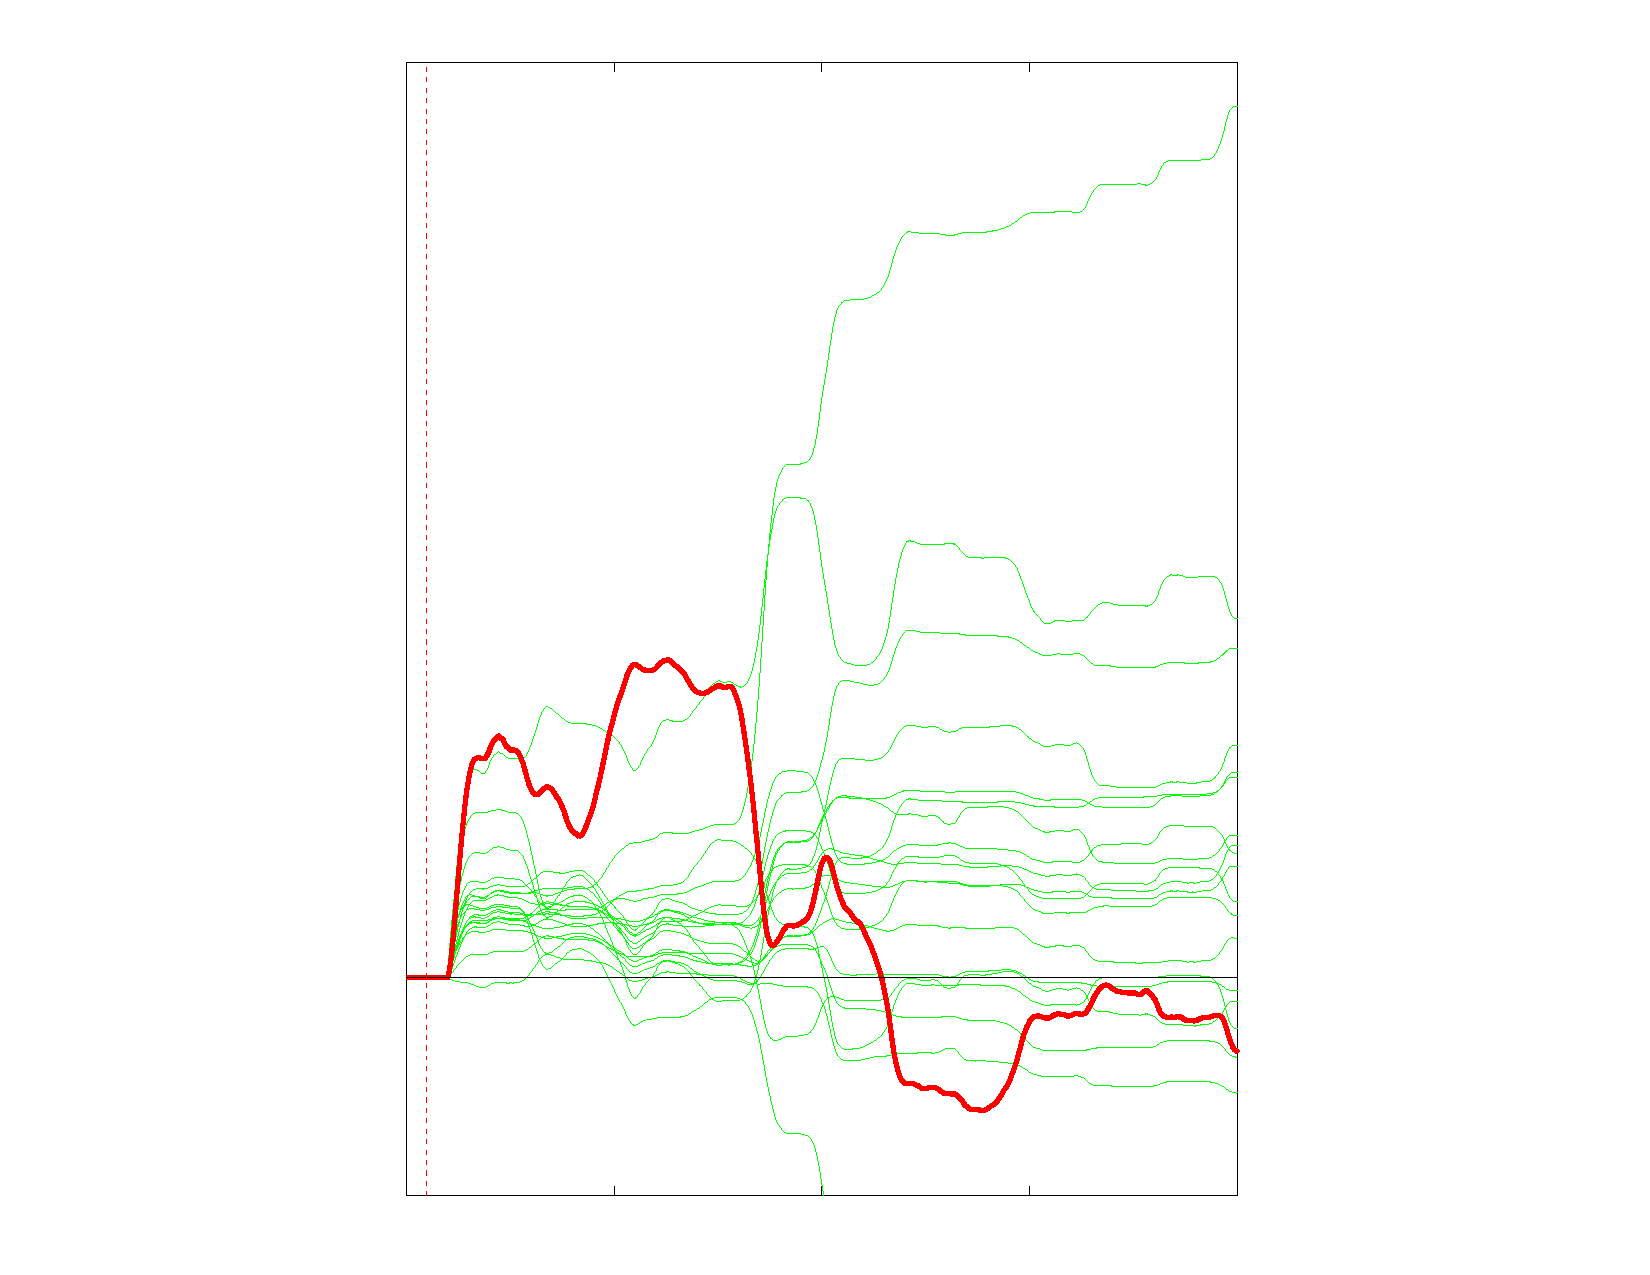
\includegraphics[trim={6.5cm 1cm 5cm 1cm},clip,width=6cm,height=3.5cm]{img/409-clusterSmallWorld-20-addUniform-40-spike-gaussian-Unobserved-fullKL-ukf-Xhat}};
\node at (0,-0.25) {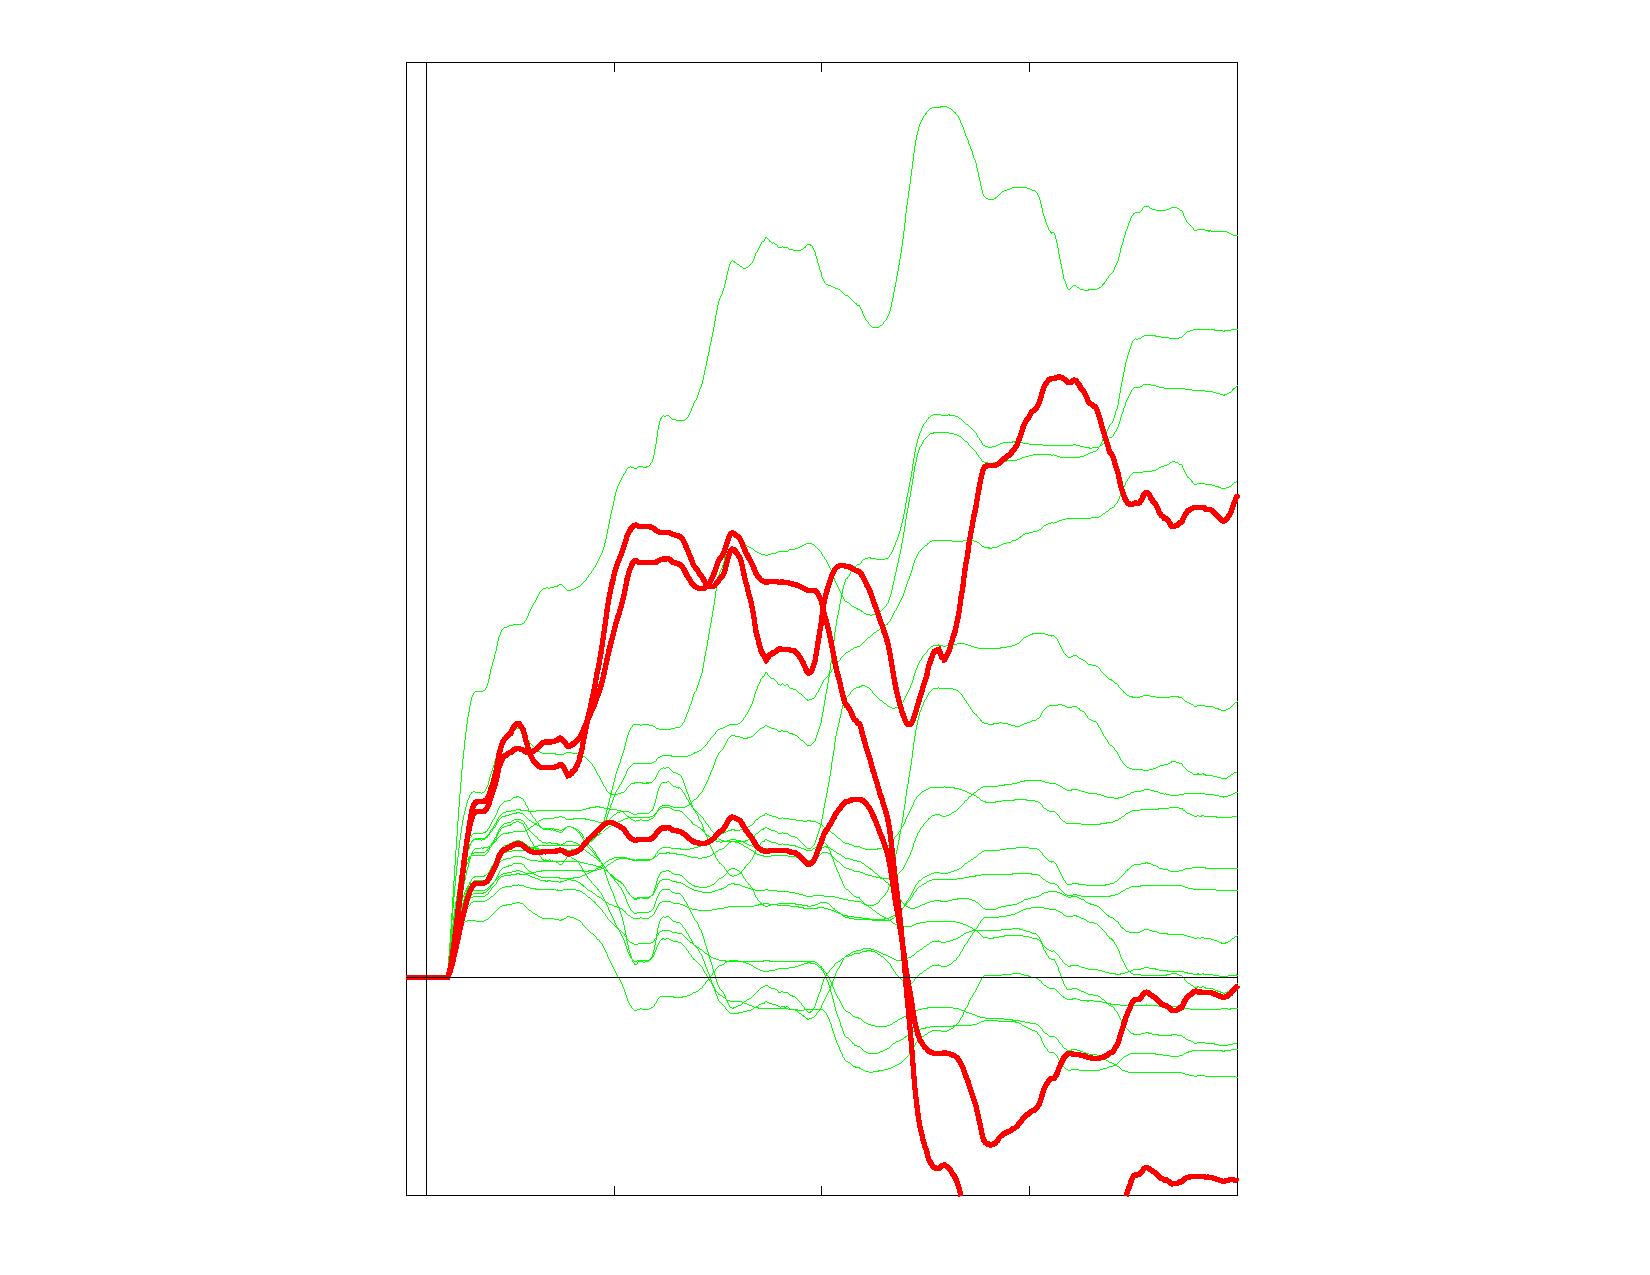
\includegraphics[trim={6.5cm 1cm 5cm 1cm},clip,width=6cm,height=3.5cm]{img/409-clusterSmallWorld-20-addUniform-40-spike3-gaussian-Unobserved-fullKL-ukf-Xhat}};
\node at (5.5,-0.25) {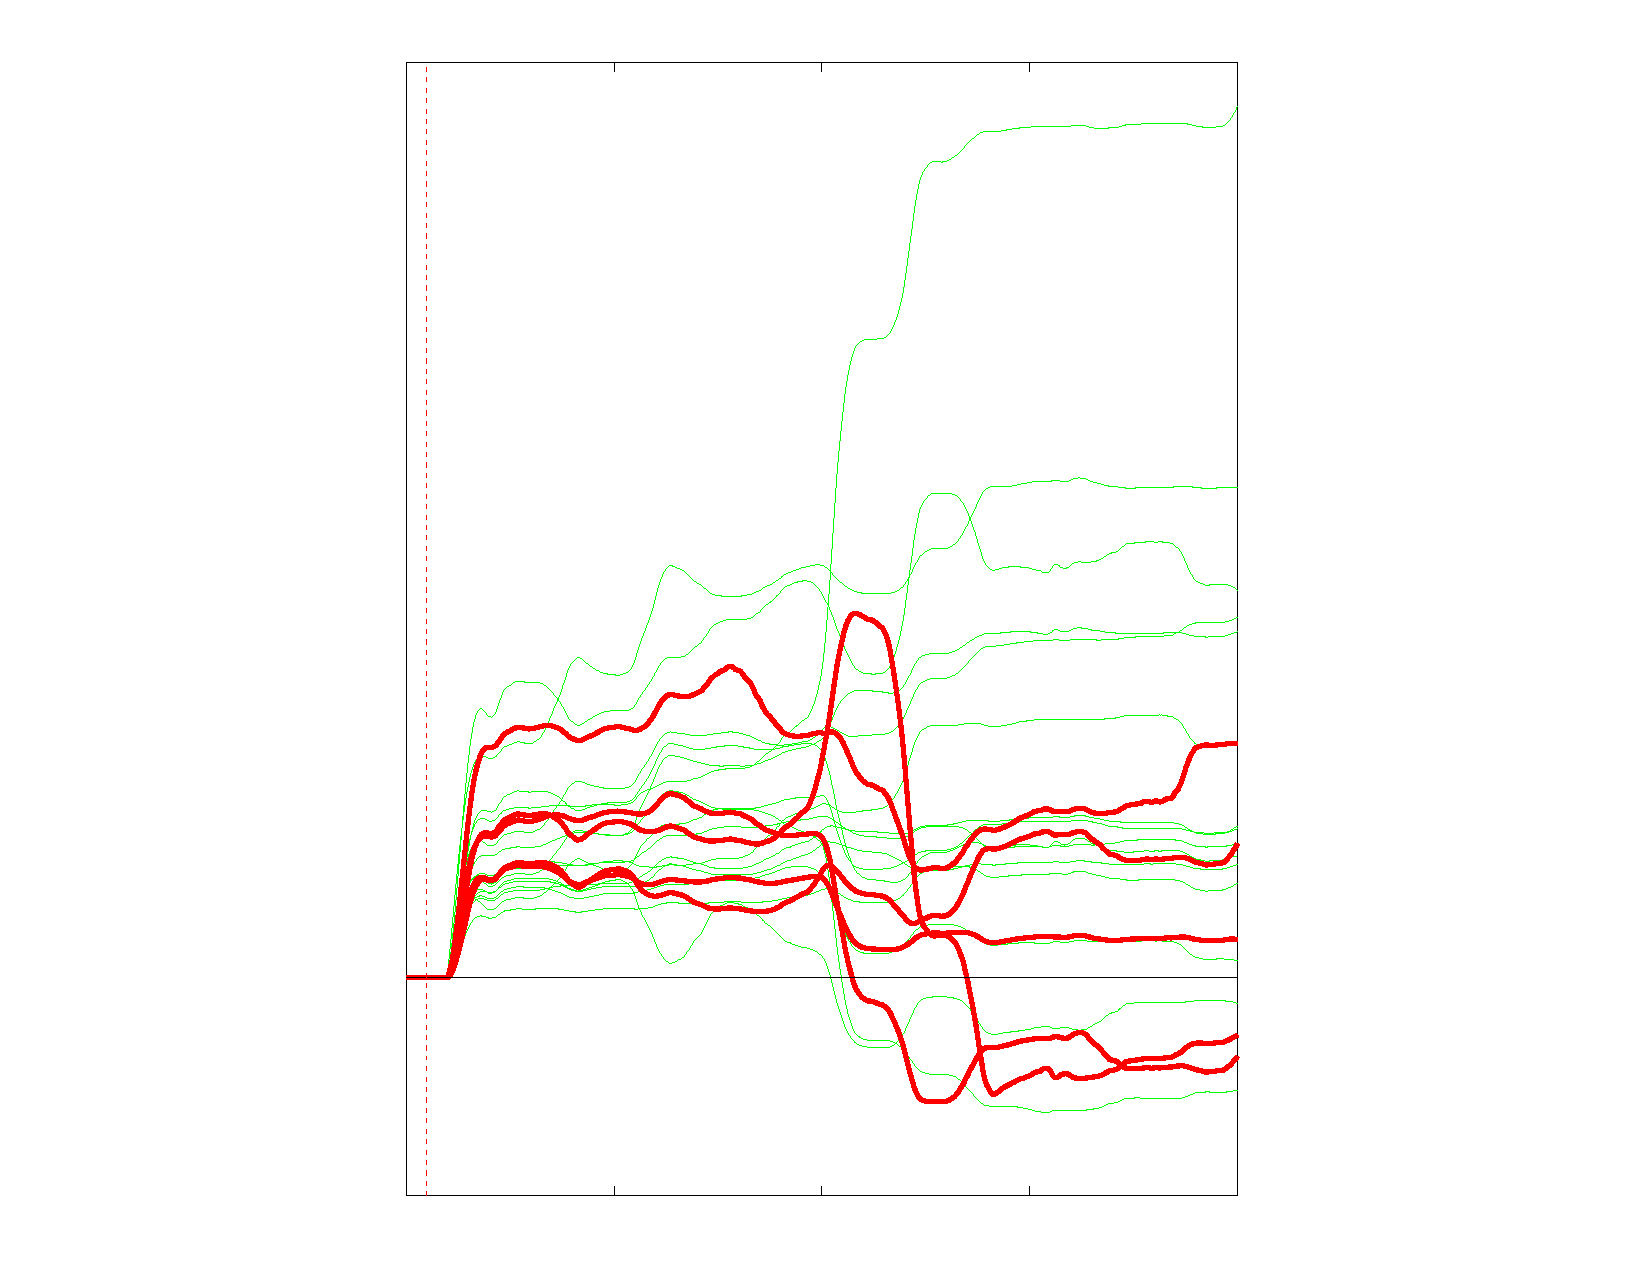
\includegraphics[trim={6.5cm 1cm 5cm 1cm},clip,width=6cm,height=3.5cm]{img/409-clusterSmallWorld-20-addUniform-40-spike5-gaussian-Unobserved-fullKL-ukf-Xhat}};

\node at (-5.5,3.6) {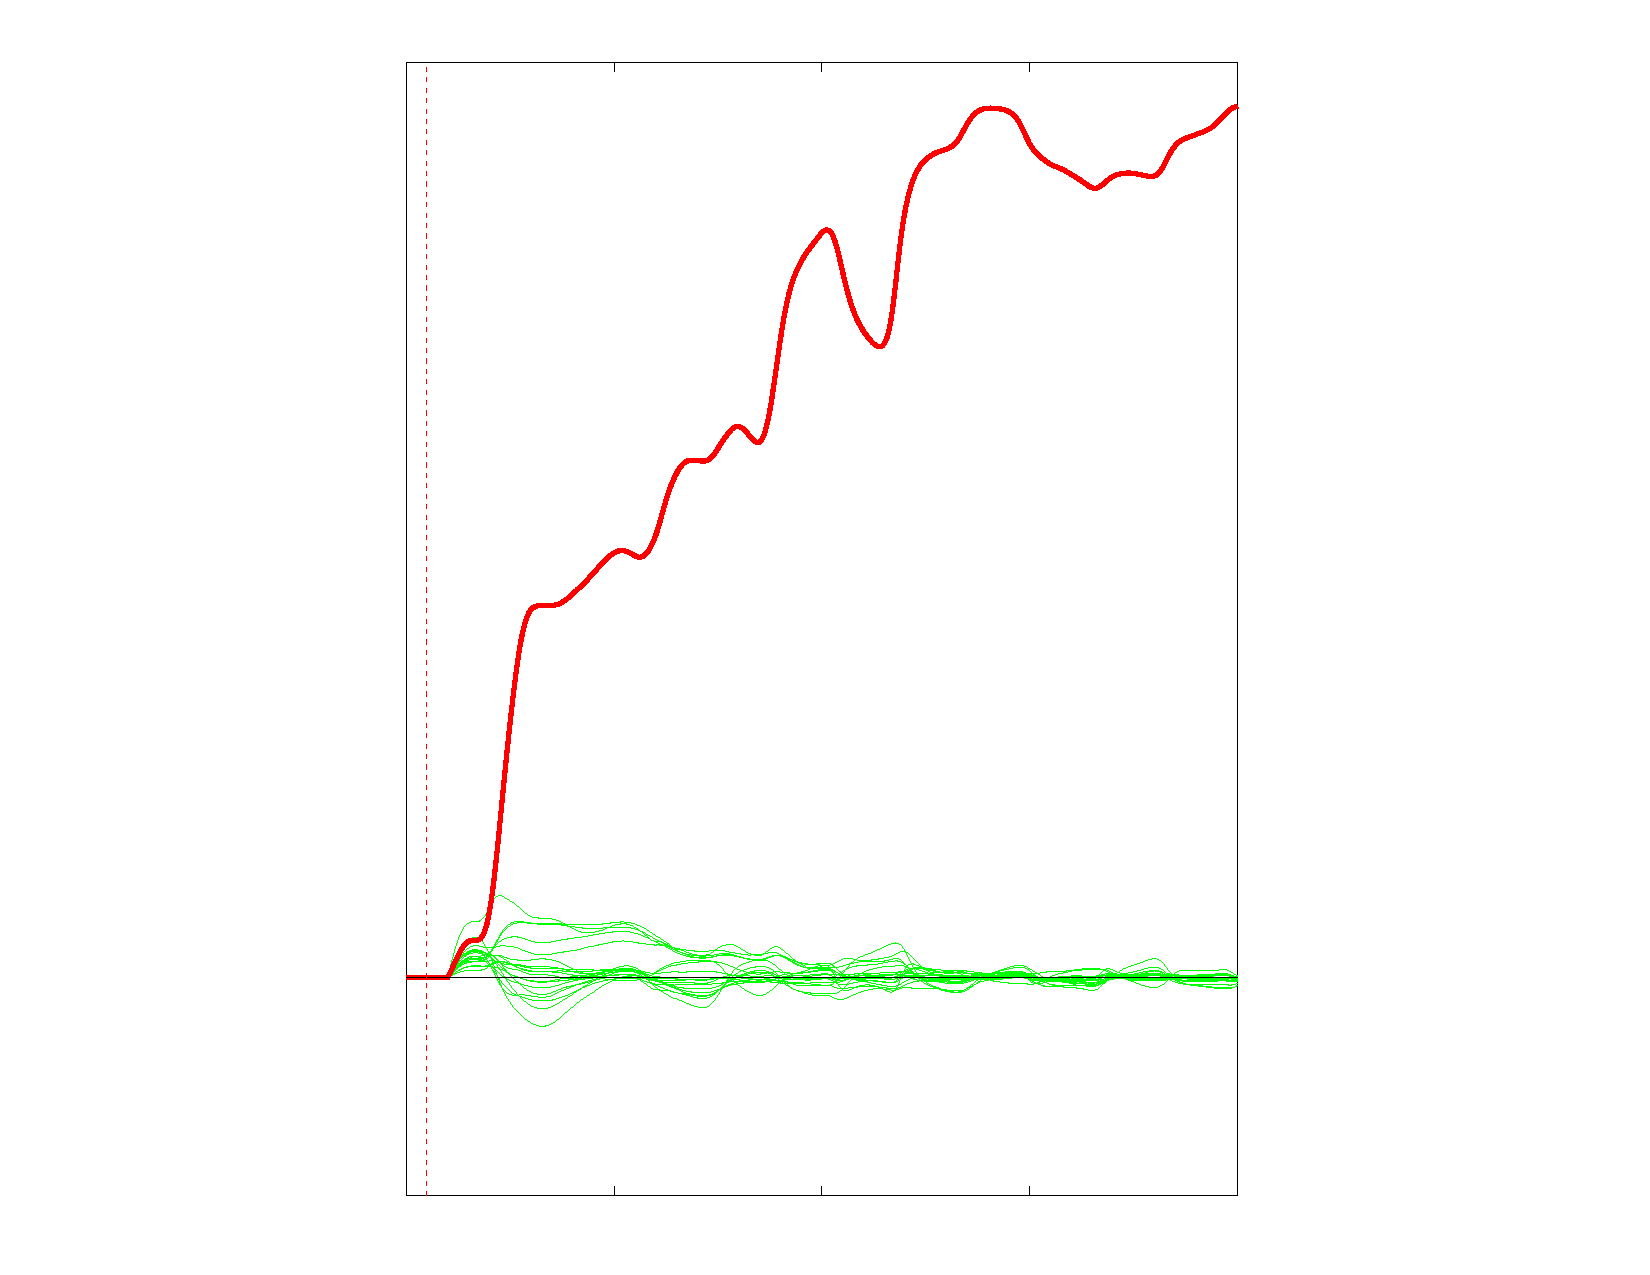
\includegraphics[trim={6.5cm 1cm 5cm 1cm},clip,width=6cm,height=3.5cm]{img/409-clusterSmallWorld-20-addUniform-40-spike-gaussian-Unobserved-rank1-ukf-Xhat}};
\node at (0,3.6) {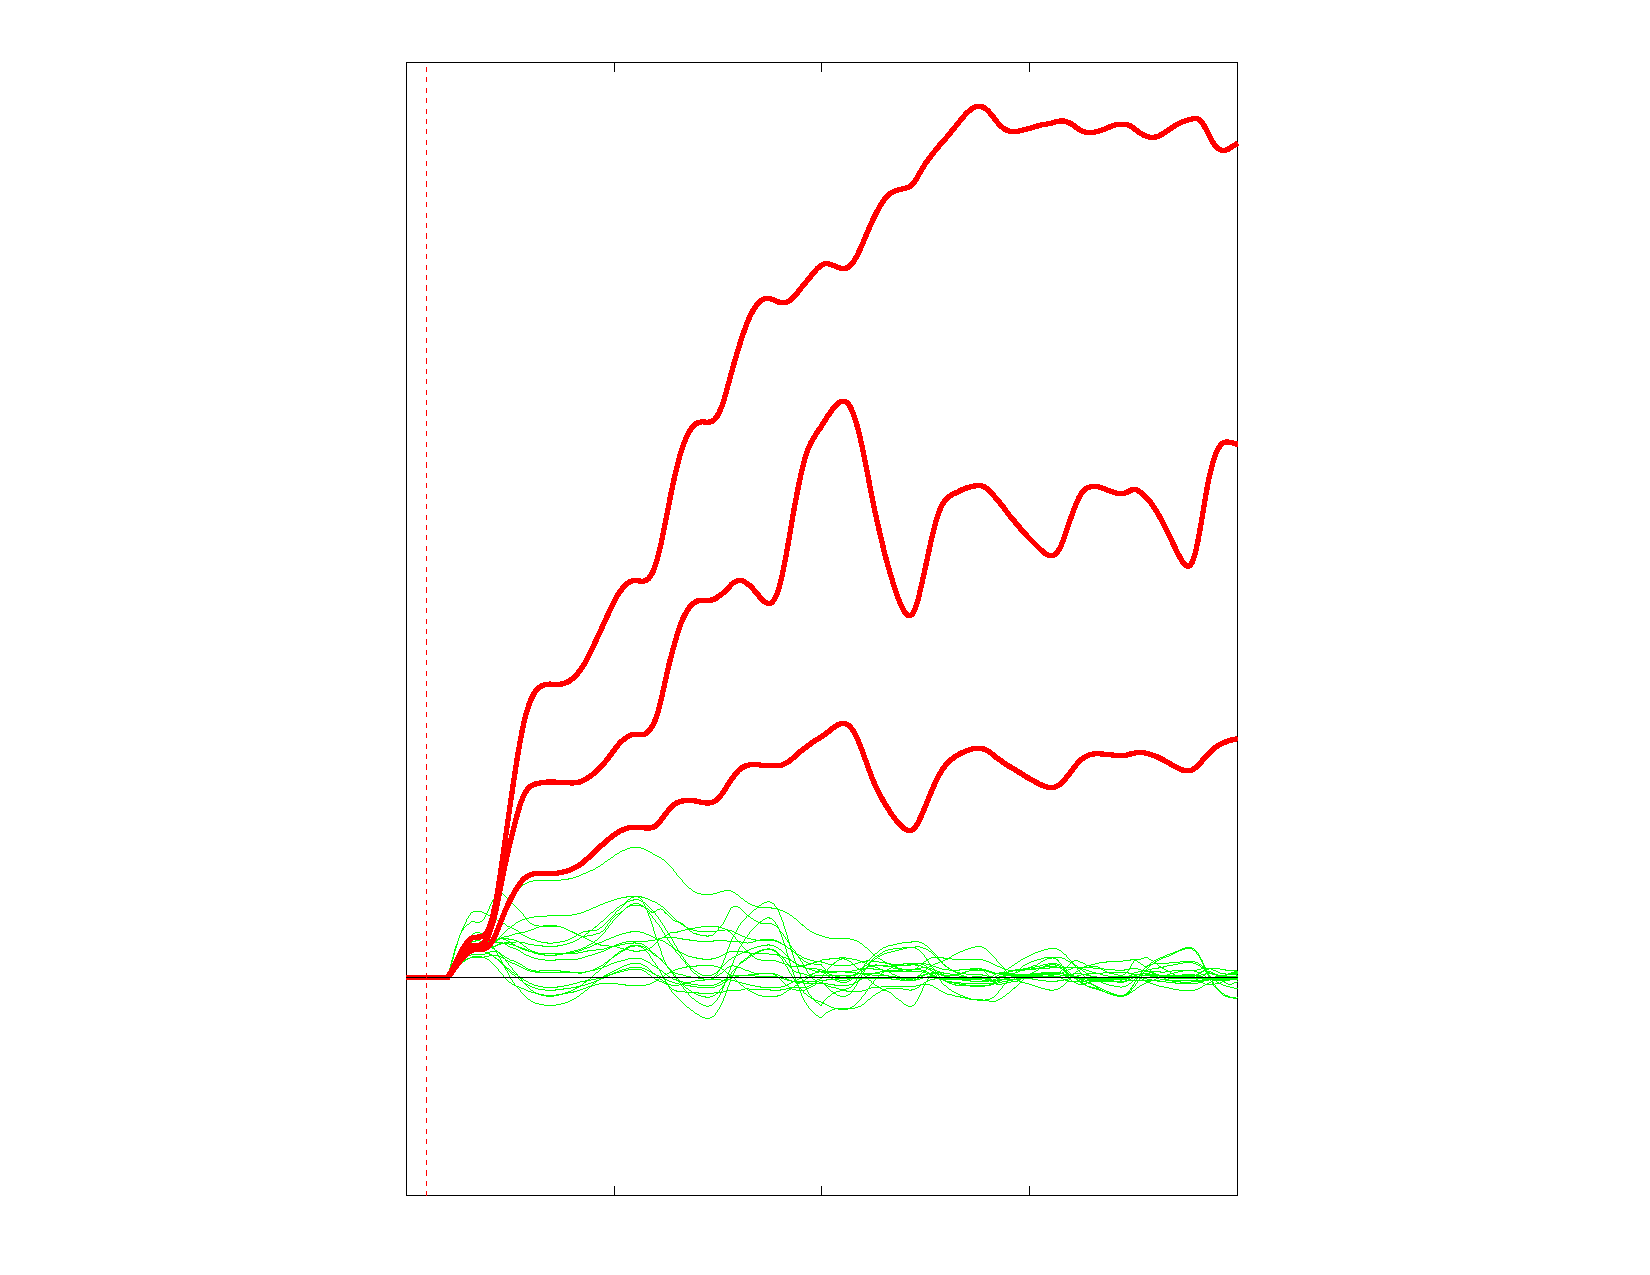
\includegraphics[trim={6.5cm 1cm 5cm 1cm},clip,width=6cm,height=3.5cm]{img/409-clusterSmallWorld-20-addUniform-40-spike3-gaussian-Unobserved-rank1-ukf-Xhat}};
\node at (5.5,3.6) {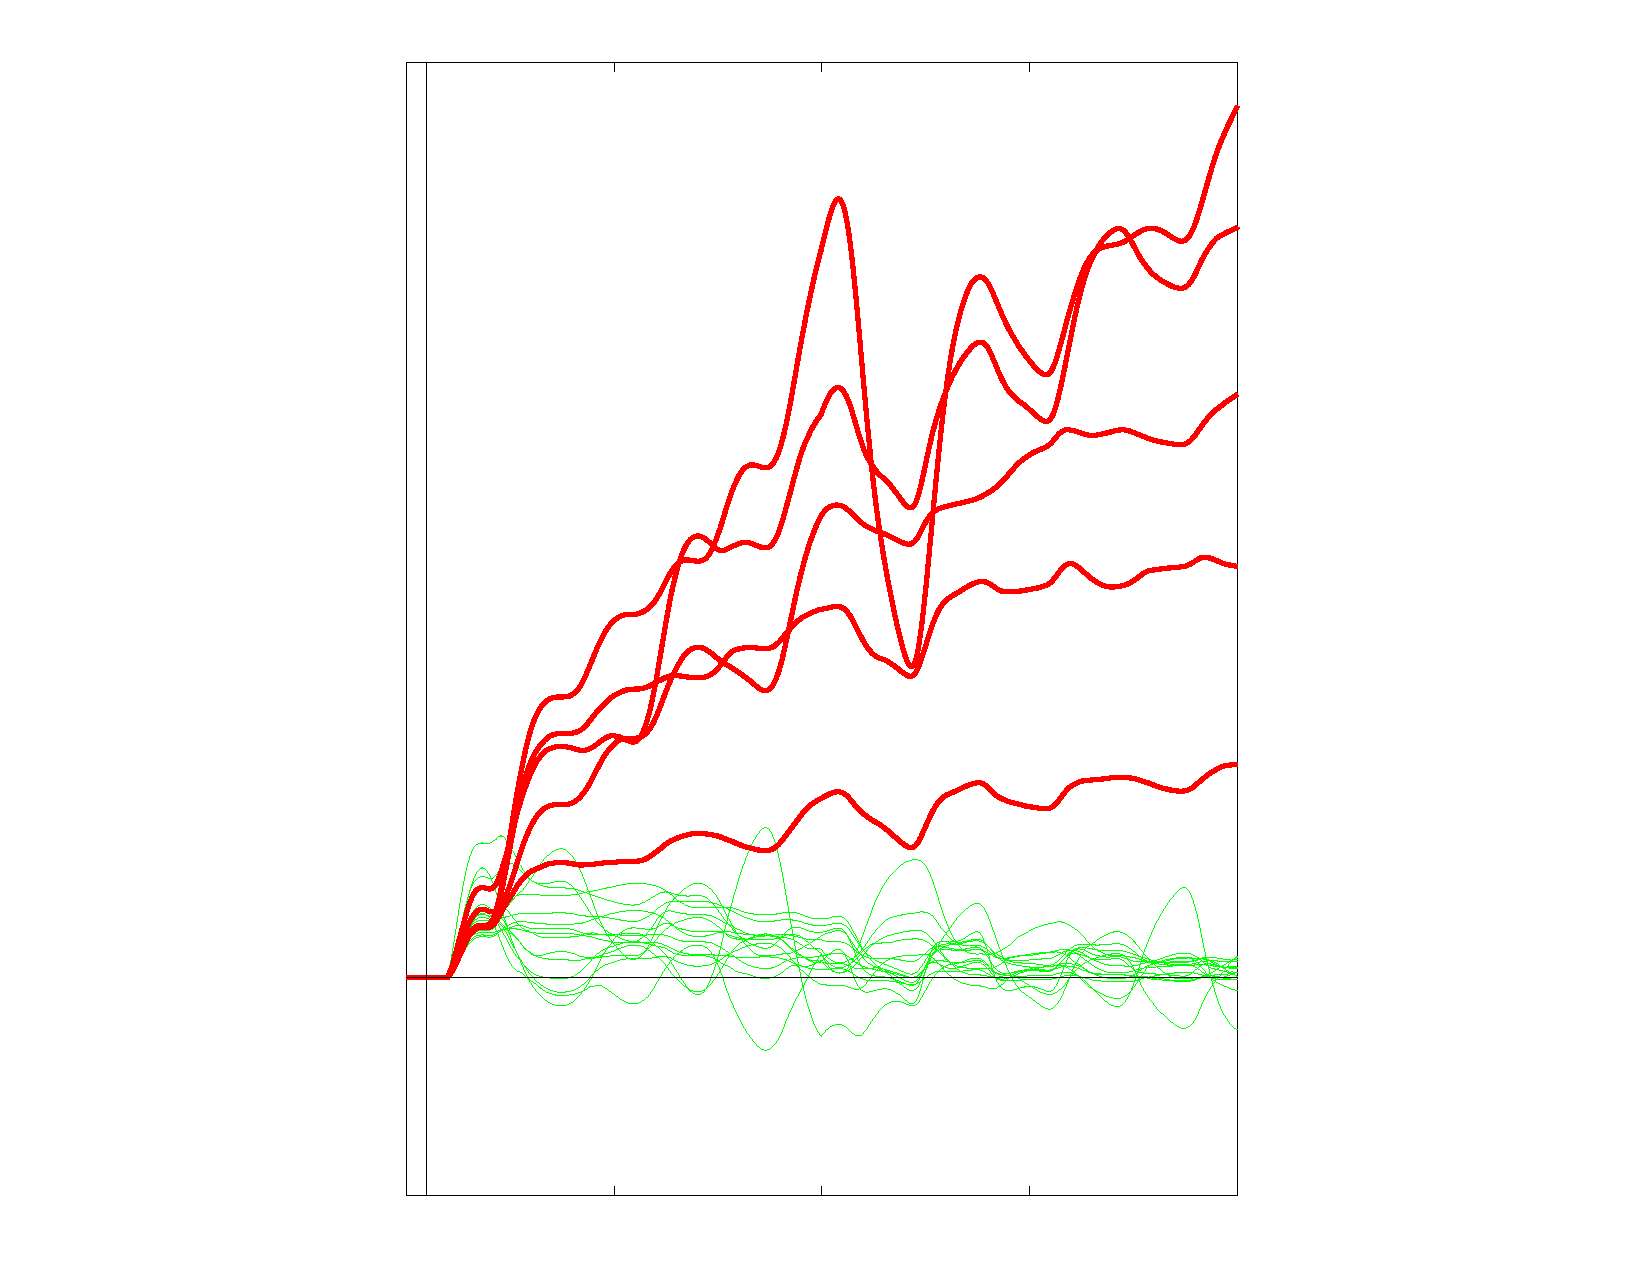
\includegraphics[trim={6.5cm 1cm 5cm 1cm},clip,width=6cm,height=3.5cm]{img/409-clusterSmallWorld-20-addUniform-40-spike5-gaussian-Unobserved-rank1-ukf-Xhat}};

\node at (-5.755,5.75) {1 compromised bus};
\node at (-0.25,5.75) {3 compromised buses};
\node at (5.25,5.75) {5 compromised buses};

\draw (-8.25,-2.65) -- (-7.30,-2.65);
\draw[->] (-4.2,-2.65) -- (7.75,-2.65);
\node at (-5.75,-2.65) {simulation time (sec)};

\node at (-8.35,-2.25) {0.0};
\node at (-7.05,-2.25) {0.5};
\node at (-5.75,-2.25) {1.0};
\node at (-4.45,-2.25) {1.5};
\node at (-3.25,-2.25) {2.0};

\node at (-6.75,1.25) {\color{darkgray} attack initiated};
\draw[->,darkgray] (-7.75,1.25) -- (-8.15,1.25);

\node at (-5,3.75) {\color{red} compromised buses};
\draw[->,red] (-6,3.95) -- (-6.15,4.15);

\node at (4.3, 1.1) {\color{darkgreen} uncompromised buses};
\draw[->,green] (5.25,0.9) -- (5.5,0.8);
\end{tikzpicture}
\caption{
    Each line in the figures above represents the predicted positive feedback of a particular load bus.
    Compromised buses are drawn in bold red,
    and uncompromised buses are drawn in thin green.
    For all times $t$ before the attack begins, each bus $i$ has $f_i(t)$ near zero.
    After the attack begins, the $f_i(t)$ deviate from zero.
    Our method is correctly identifying the attacked buses whenever the red lines are above the green lines.
    In the top row, we see that our rank-1 approximation of $K^{LG}$ provides relatively accurate predictions even when the number of attacks increases and the rank-1 approximation is no longer true.
    In the bottom row, we see that the standard method has poor accuracy.
}
\label{fig:destab}
\end{figure*}

All experiments in this section use a single randomly generated power grid with 20 generator and 20 load buses.
We test on this relatively small grid size because the standard method estimates a full rank $K^{LG}$ matrix cannot scale to larger problems.
On this size problem, a single iteration of our rank-1 method takes about 1 second,
and a single iteration of the standard method takes about 1 minute.
On a problem with 100 generators and 100 loads,
a single iteration of our rank-1 method takes about 5 seconds,
and a single iteration of the standard method takes over an hour.
The computation advantage of our proposed method is evident.

We follow the \emph{clusterSmallWorld} procedure for generating the power grid \cite{wang2010generating}. Note that, standard methods for generating random graphs do not exhibit the topological and electrical properties of real world power grids \cite{hines2010topological},
but \emph{clusterSmallWorld} was designed specifically for modeling real world power grids.
An outline of the procedure is:
First generate a random number of ring shaped grids with fewer than 10 buses each;
Then randomly add connections between the buses until the average degree of each node is 4.
To ensure the stability of the resulting system,
scale matrix $A$ so that its maximum eigenvalue is no greater than 0.999.
This model generates realistically shaped power grids up to about 300 buses.
Once the power grid has been generated, a load input vector, i.e., $\uu_t$, is sampled from a Gaussian process truncated so that values are always non-negative.

The first experiment has 6 separate scenarios that test how the proposed method and the standard method perform in identifying 1, 3, and 5 compromised buses.
In each case, the attack begins at time 0.1 seconds.
Matrix $A^p_t$ is selected such that $(A+BA^p_t)$ has maximum eigenvalue 1.05,
ensuring that the attack destabilizes the system.
Figure $\ref{fig:destab}$ shows the results.
The proposed method clearly has better qualitative performance on this particular problem. Specifically, it identifies the compromised buses faster and more accurately.


To look carefully into how our proposed method can differentiate between benign and malicious loads, next we randomly selected a load $i$ and generator $j$, then set the $i$th row and $j$th column of ${K^{LG}}$ to $-10$.
Recall that negative values of the $K^{LG}$ matrix correspond to benign loads.
The results are shown in Figure \ref{fig:neg}.
Negative feedback does not destabilize the system,
yet we are able to detect the feedback.
The standard method (not shown) has difficulty with this problem as it takes much longer for the standard method to converge.

\begin{figure}
\begin{tikzpicture}
\small
\node at (0,0) {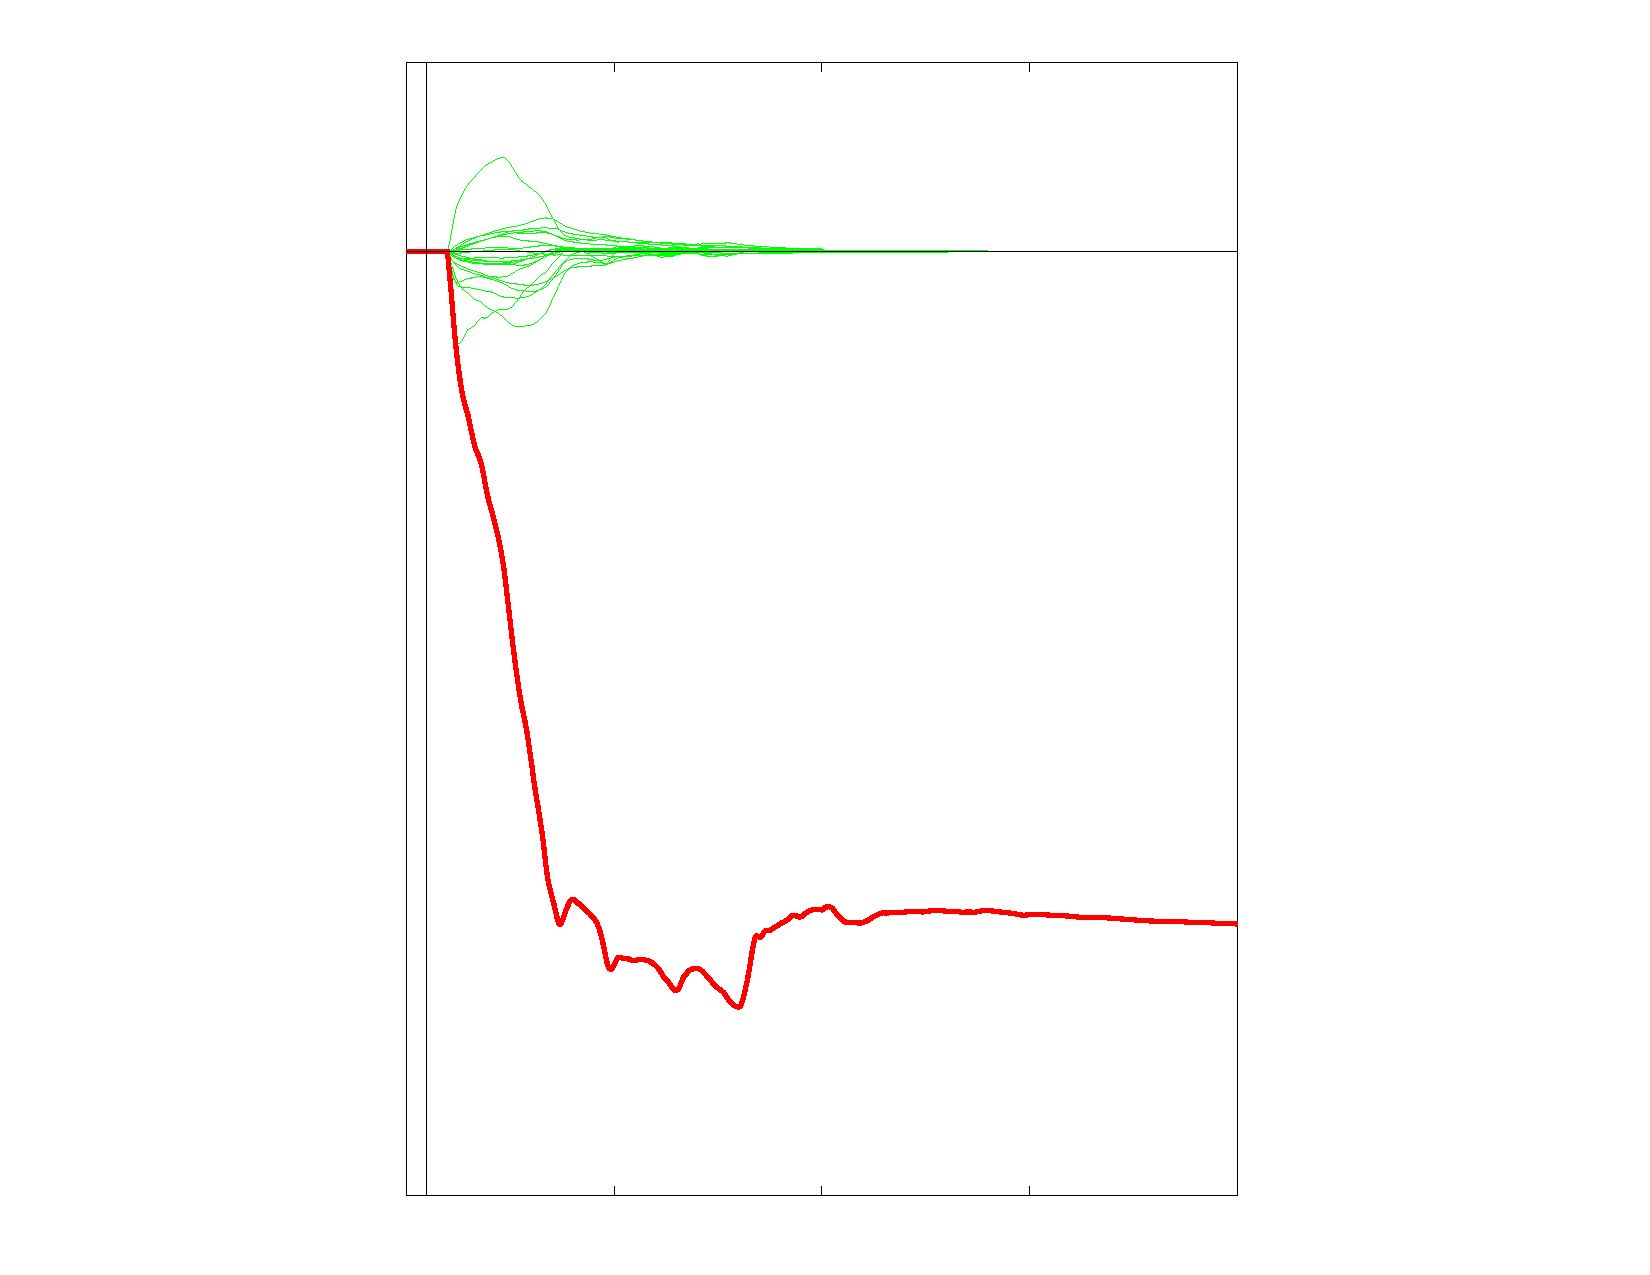
\includegraphics[trim={6.5cm 1cm 5cm 1cm},clip,width=8cm,height=4.5cm]{img/406-clusterSmallWorld-20-addUniform-40-spikeNeg-gaussian-Unobserved-rank1-ukf-Xhat}};
\node at (-0.35,-2.95) {simulation time (sec)};
\node at (-4.5,0) {\rotatebox{90}{$f_i(t)$}};

\node at (-3.8,-2.5) {0.0};
\node at (-2.05,-2.5) {0.5};
\node at (-0.35,-2.5) {1.0};
\node at (1.35,-2.5) {1.5};
\node at (3.05,-2.5) {2.0};

\node at (-1.75,-1.8) {\color{darkgray}responsive load added};
\draw[->,darkgray] (-3.25,-1.75) -- (-3.5,-1.75);

\node at (1,-0.8) {\color{red}bus with responsive load};
\node at (-1,1.8) {\color{darkgreen}buses with normal loads};

\end{tikzpicture}
\caption{
    In this simulation, we added a benign frequency responsive load.
    %In this simulation, negative feedback has been added to the system.
    %We see that our estimates of $f_i$ correctly go negative.
    Our rank-1 method is able to quickly identify the load with the responsive feedback.
    The corresponding value of $f_i(t)$ is negative because the feedback is negative.
    Previous work cannot distinguish these benign frequency responsive loads from malicious loads,
    whereas ours can.
    }
\label{fig:neg}
\end{figure}

\subsection{Quantitative Results}

We now explore the quantitative performance of our methods by measuring its performance on several power systems.
We generated two sets of power grids, one with 20 generators and 20 loads (as in the previous section), and the other one with 100 generators and 100 loads.
The standard method was run only on the smaller grid, again because it is computationally infeasible to run it on the larger one, and the proposed method was run only on both grids.

A major strength of both methods is that they experienced no false positives.
We define a false positive to be the detection of an attack when no attack occurred. It does not matter if the value of $\alpha_t$ is correct.
When no attack is underway, the largest entries of the estimated $K^{LG}_t$ are typically less than $10^{-6}$.
When an attack is underway, the largest values of the estimated $K^{LG}$ skyrocket to well above $10^{-1}$.
Therefore, it is easy to set the threshold $\tau$ to avoid false positives.

Finally, we evaluate the method's \emph{accuracy of identification}.
We define the accuracy at time point $t$ to be the fraction of $\alpha_t$ values that correctly predict the attacked bus.
Figure \ref{fig:accuracy} shows that the longer we wait to declare an attack occurs
(i.e. the larger we set $\tau$), the higher our accuracy is.
In the case of the rank-1 method detecting a single attack,
we observed $99\%$ accuracy in under one second.
The rank-1 method operating on the 200 bus system has much higher accuracy than the standard method operating on the significantly easier 40 bus system.
The standard method's accuracy is little better than random guessing after two seconds.

%The next important measure is the method's accuracy.
%That is, when we identify an attack
%First, we want to emphasize that our method has an essentially zero false positive rate.
%
%For the first experiment, we measured

\begin{figure}
%\begin{tabular}{cc}
%\begin{turn}{90}
%~~~~~~~~~~~~~accuracy of $\alpha_t$
%\end{turn}
%&
%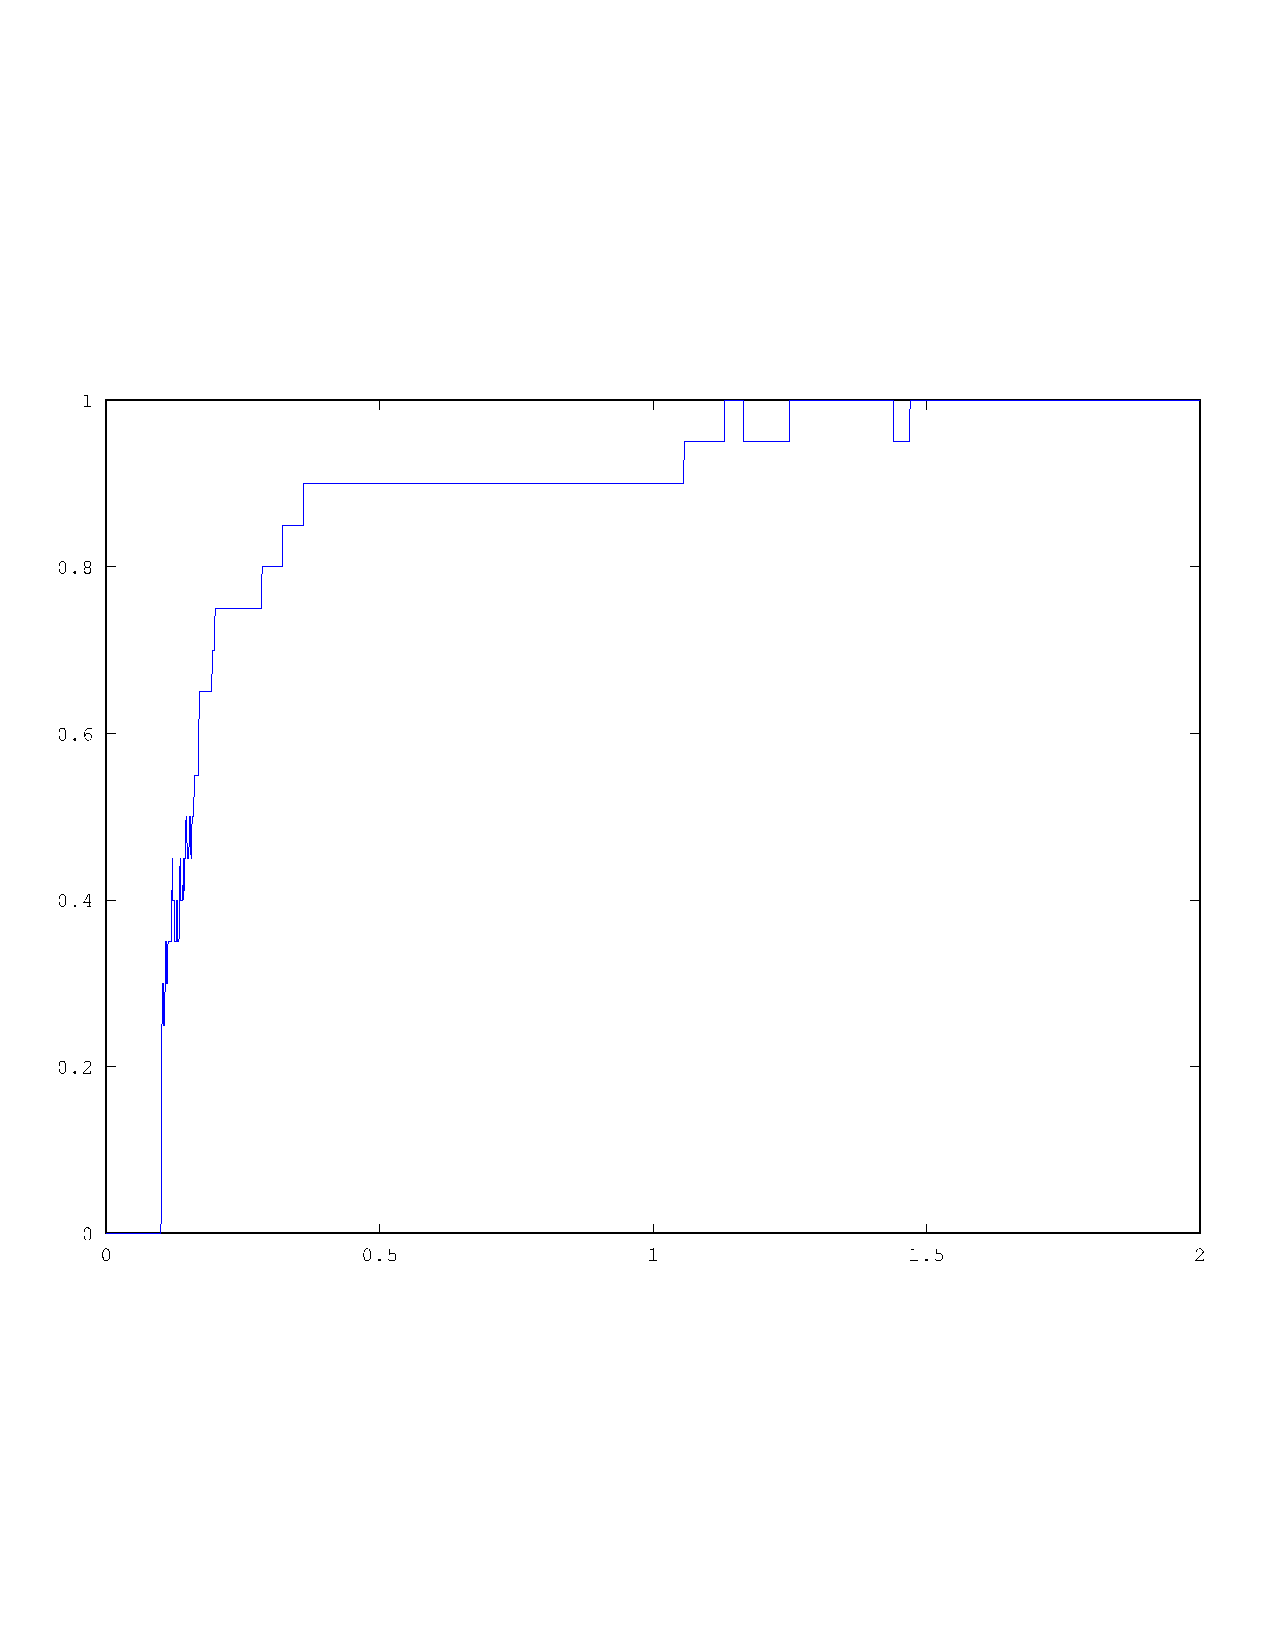
\includegraphics[width=0.4\textwidth, trim= 0 2in 0 2in, clip]{img/clusterSmallWorld-100-addUniform-400-spike-gaussian-Unobserved-rank1-ukf-fraction}
%\\
%& time
%\end{tabular}
\begin{tikzpicture}
\small
\node at (-0.1,0) {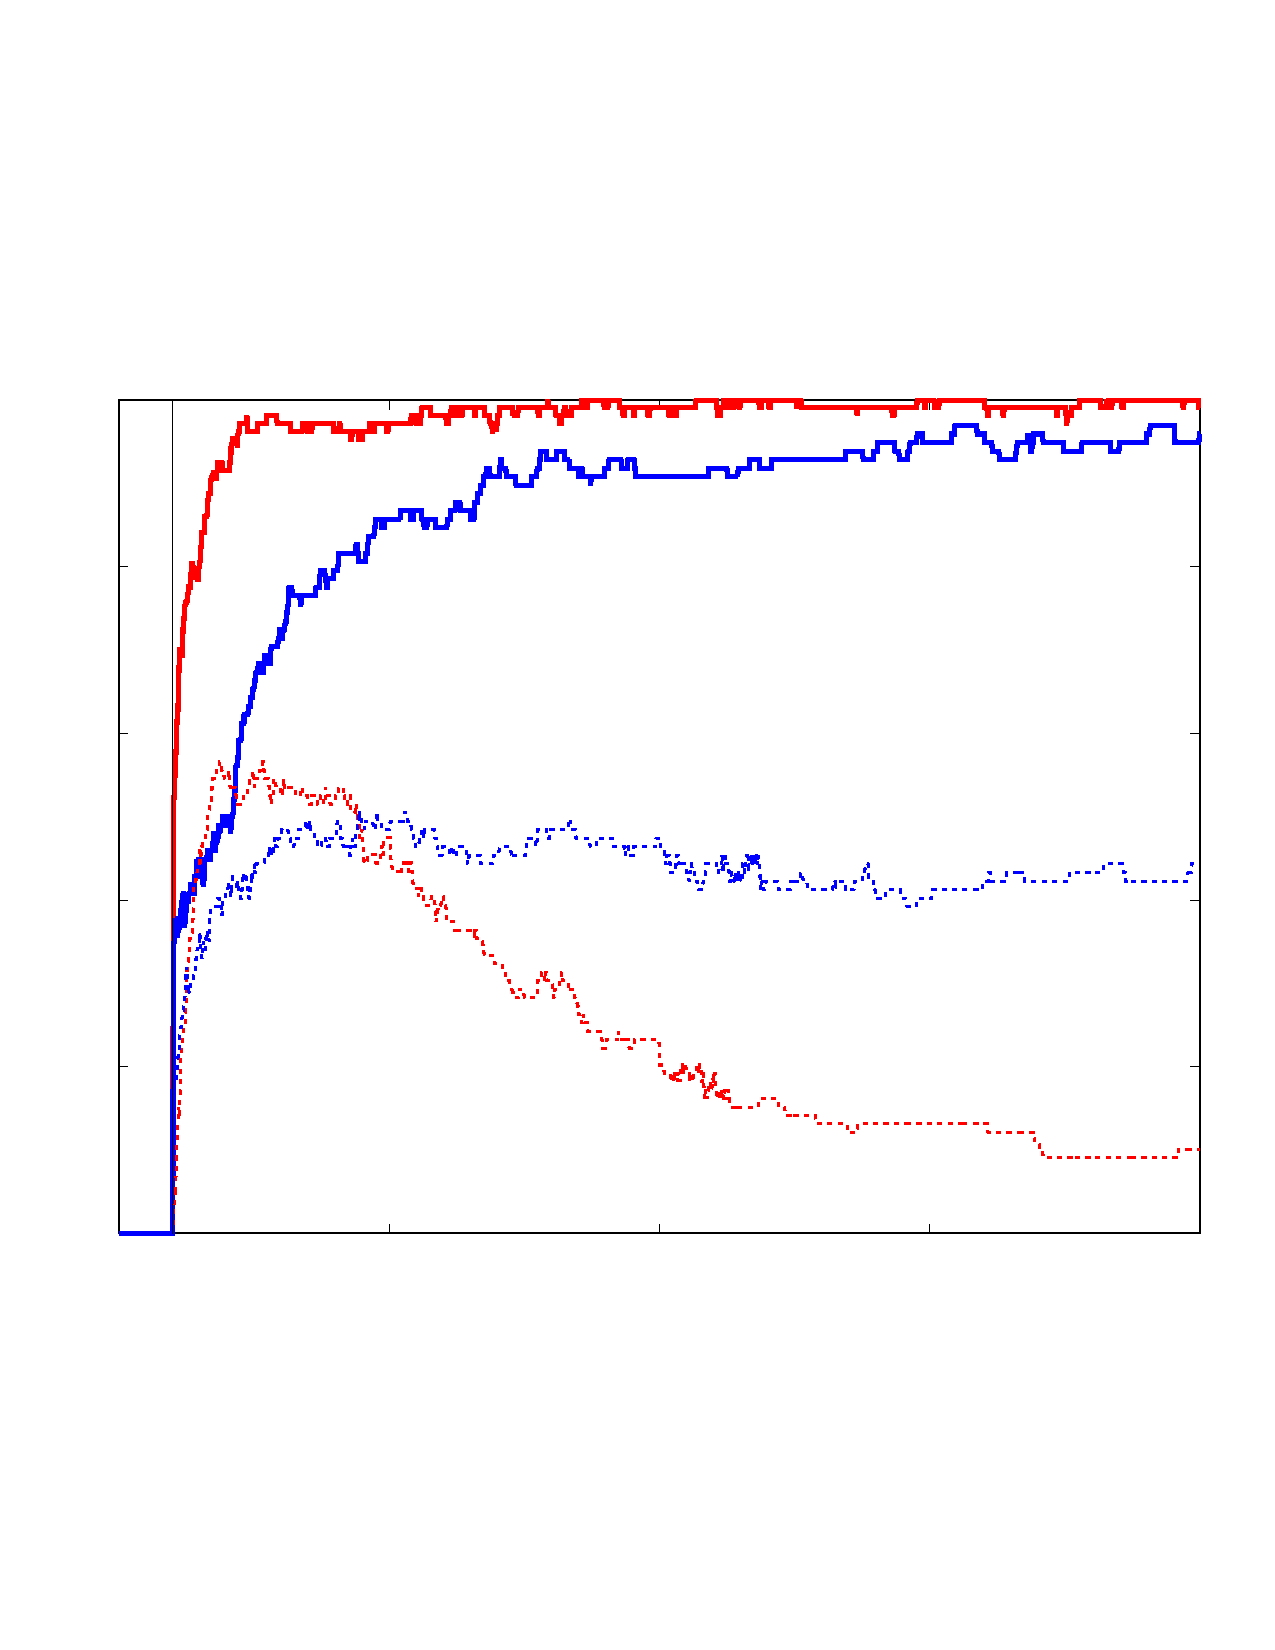
\includegraphics[trim={2cm 5cm 1cm 5cm},clip,width=7.2cm,height=7cm]{img/accuracy}};
\node at (0.0,-3.5) {simulation time (sec)};
\node at (-4.7,0) {\rotatebox{90}{accuracy of $\alpha_t$}};

\node at (-3.65,-3) {0.0};
\node at (-1.85,-3) {0.5};
\node at (-0.1,-3) {1.0};
\node at (1.65,-3) {1.5};
\node at (3.45,-3) {2.0};

\node at (-4.1,-2.7) { 0.0 };
\node at (-4.1,-1.6) { 0.2 };
\node at (-4.1,-0.5) { 0.4 };
\node at (-4.1,0.55) { 0.6 };
\node at (-4.1,1.65) { 0.8 };
\node at (-4.1,2.8) { 1.0 };

\node at (-1.9,-2.2) {\color{darkgray}attack initiated};
\draw[darkgray,->] (-2.9,-2.2) -- (-3.3,-2.2);

\node at (2,-1.5) {\color{red}\begin{tabular}{c}full $K^{LG}$\\1 compromised bus\end{tabular}};

\node at (2,0.25) {\color{blue}\begin{tabular}{c}full $K^{LG}$\\5 compromised buses\end{tabular}};

\node at (2,1.95) {\color{blue}\begin{tabular}{c}rank-1 $K^{LG}$\\5 compromised buses\end{tabular}};

\node at (-1.75,3.25) {\color{red}\begin{tabular}{c}rank-1 $K^{LG}$\\1 compromised bus\end{tabular}};

\end{tikzpicture}
\caption{
    It takes only about a quarter of a second for our rank-1 method to detect a single attack with 99\% accuracy.
    As the number of attacks increases, our rank-1 method takes longer to achieve high accuracy.
    With 5 compromised buses, the attack is detected with 95\% accuracy by two seconds.
    This is fast enough to implement corrective actions.
    The full $K^{LG}$ method has much worse accuracy no matter how many buses are compromised.
}
\label{fig:accuracy}
\end{figure}

%\begin{figure}
%\begin{tabular}{cc}
%\begin{turn}{90}
%~~~~~~~~~~threshold
%\end{turn}
%&
%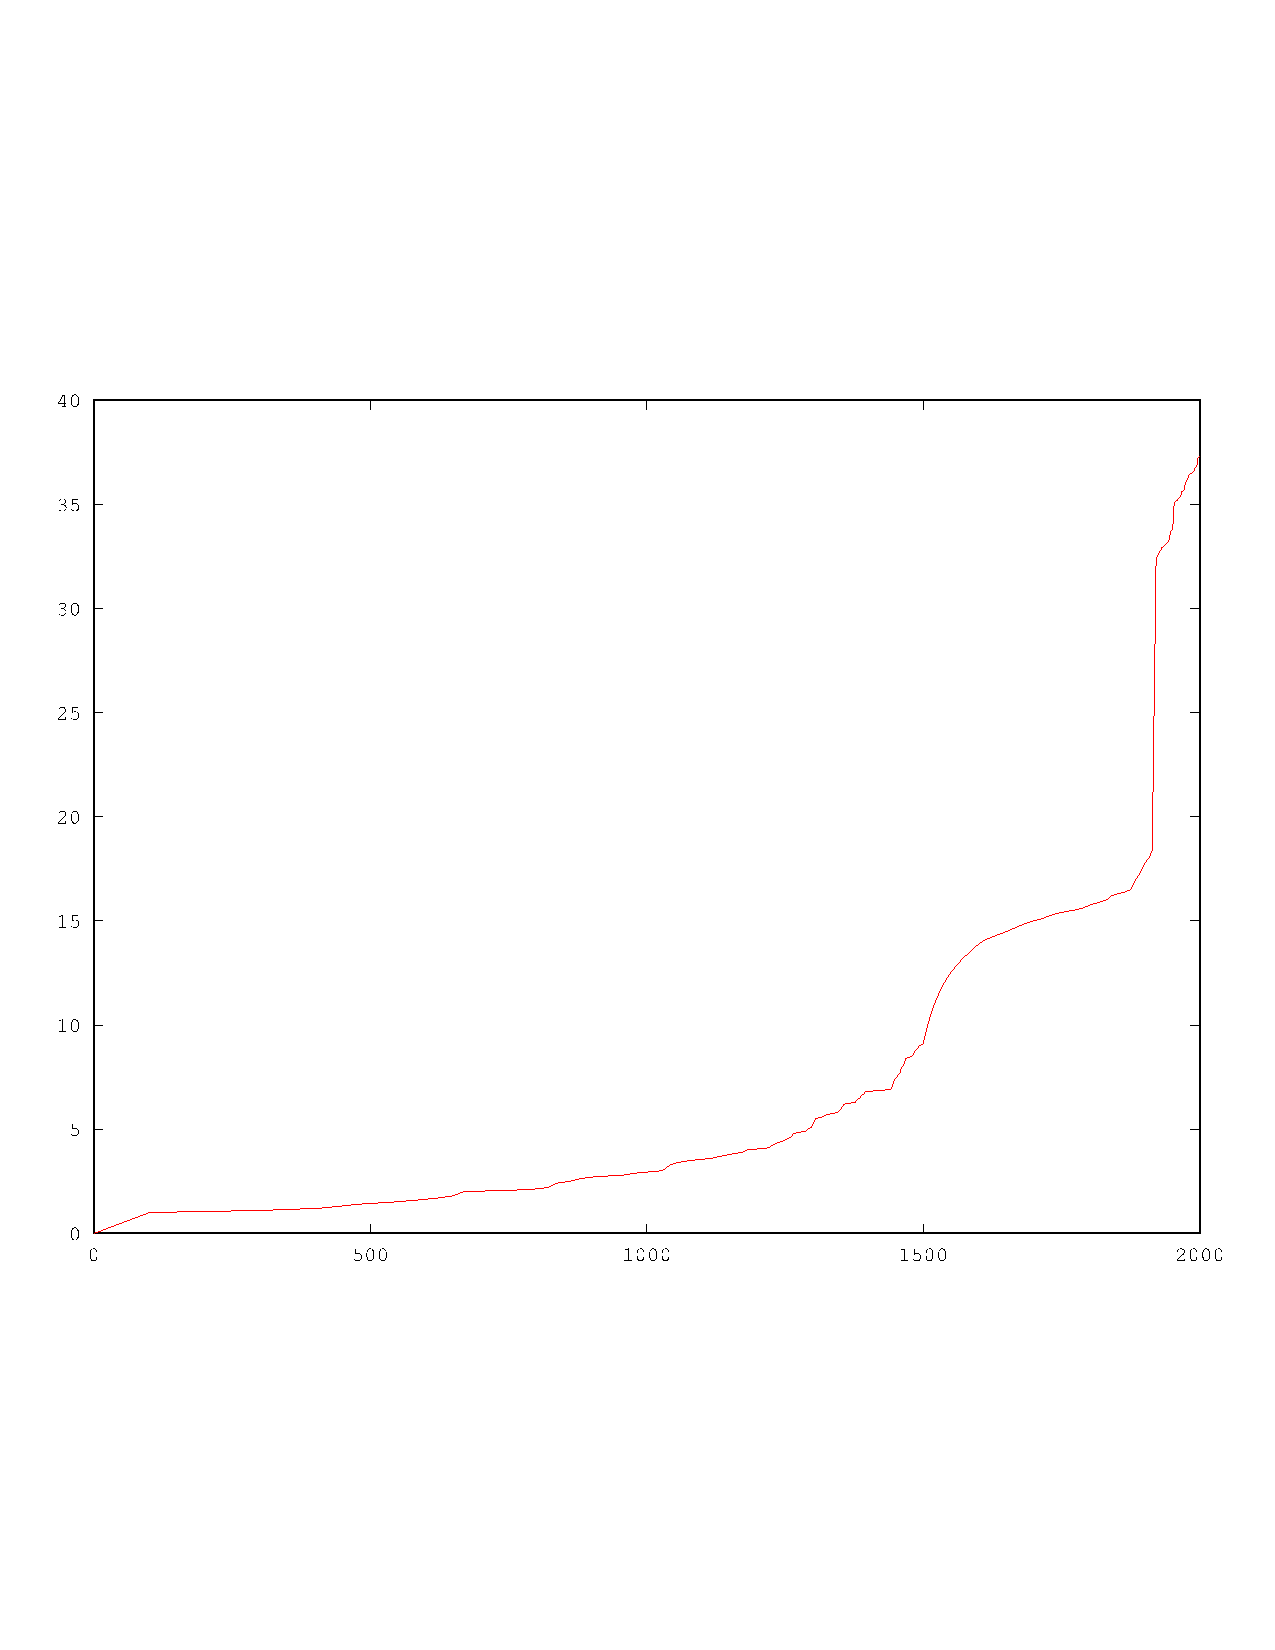
\includegraphics[width=0.4\textwidth, trim= 0 2in 0 2in, clip]{img/clusterSmallWorld-100-addUniform-400-spike-gaussian-Unobserved-rank1-ukf-thresholds}
%\\
%&
%time
%\end{tabular}
%\caption{
    %This plot shows the average time to first detection of an attack as a function of the threshold value.
%}
%\label{fig:threshold}
%\end{figure}

%%%%%%%%%%%%%%%%%%%%%%%%%%%%%%%%%%%%%%%%%%%%%%%%%%%%%%%%%%%%%%%%%%%%%%%%%%%%%%%%

\section{Conclusions}

In this paper we addressed the open problem of detecting a destabilizing attack against the power system, i.e., identifying which buses are compromised through a possible positive feedback. Our method does not require prior knowledge on the number of buses that are compromised. It also does not require conducting a separate analysis at each bus. Instead, it naturally identifies attacks on the entire system considered as a whole. Therefore, it has low computational complexity. Furthermore, it is capable of distinguishing destabilizing attacks, i.e., load or generation control loops that are malicious and based on positive feedback, from the many load and generation control loops that exist in a power system that are benign and based on negative feedback.  Numerical results show that this method successfully identifies complex attacks involving many buses. The  detection is accurate and fast.



\bibliographystyle{plain}
\bibliography{paper}
\end{document}
